\documentclass[12pt, a4paper]{report}
\usepackage{style}


\title{Uncertainty In Artificial Intelligence \\ \textit{Theory}}
\author{Christian Rossi}
\date{Academic Year 2023-2024}

\begin{document}

\maketitle

\newpage

\begin{abstract}
    The topics of the course are:
    \begin{itemize}
        \item Uncertainty sources that affect models: typology, issues, and modeling approaches.
        \item Measure-based uncertainty modeling.
        \item Logic-based uncertainty modeling.
        \item Fuzzy models: fuzzy sets, fuzzy logic, fuzzy rules, motivations for fuzzy modeling, tools for fuzzy systems, design 
            of fuzzy systems, applications.
        \item Bayesian networks: basics, design, learning, evaluation, applications.
        \item Hidden Markov Models: basics, design, learning, evaluation, applications.
        \item Applications: motivations, choices, models, case studies.
    \end{itemize}
\end{abstract}

\newpage

\tableofcontents

\newpage

\chapter{Introduction}
    \section{Definition}
    \begin{definition}
        \emph{Uncertainty} pertains to epistemic situations that involve imperfect or unknown information. 
        It is relevant to predictions of future events, existing physical measurements, or the unknown.
    \end{definition}
    Uncertainty can manifest in partially observable or stochastic environments, as well as stemming from ignorance, inaction, or a combination of both. 
    This concept of uncertainty is prevalent across a wide array of disciplines, such as insurance, philosophy, physics, statistics, economics, finance, medicine, psychology, sociology, engineering, metrology, meteorology, ecology, and information science.
    
    Uncertainty represents a state of incomplete knowledge, characterized by the impossibility of precisely defining the current state, a future result, or multiple potential outcomes. 
    This underscores the connection between uncertainty and the necessity to describe an aspect of reality.

    \section{Modelling}
    Modeling forms the foundation of our existence. Our interaction with the world relies on models that interpret data from sensors, yielding knowledge and guiding actions. 
    Moreover, modeling is the means by which we can represent entities in a computer and facilitate reasoning about them.
    \begin{definition}
        A \emph{model} is a representation of an entity, defined for a particular purpose. A model includes only the relevant aspects of the modeled entity. 
        It's important to note that a model inherently differs from the entity being modeled, giving rise to various forms of uncertainties within the modeling process.
    \end{definition}
    Every Artificial Intelligence application relies on models, which can be either defined by someone or learned. These models are represented in various ways, but they commonly struggle with uncertainties, primarily concerning their inputs.

    \section{Uncertainty classification}
    Uncertainty can be categorized into two primary types:
    \begin{itemize}
        \item Epistemic uncertainty: this arises from factors that, in theory, could be known but are not known in practice. 
            This can result from inaccurate measurements, overlooked model effects, or intentional data concealment. 
            Epistemic uncertainty, also termed systematic uncertainty, is, in principle, reducible by enhancing the model.   
        \item Aleatoric uncertainty: this pertains to unknown unknowns that vary each time the same experiment is conducted. 
            Aleatoric uncertainty, also referred to as statistical uncertainty, can only be described using statistical information. 
            It may also be influenced by data acquisition and processing methods. 
            In general, it is present when the model lacks comprehensive coverage.
    \end{itemize}
    The sources of uncertainty can be classified into several categories:
    \begin{itemize}
        \item Parameter uncertainty: arising from model parameters with exact values unknown to experimentalists and beyond experimental control, or whose values cannot be inferred through statistical methods.
        \item Parametric variability: stemming from the variability in input variables of the model. 
        \item Structural uncertainty: also referred to as model inadequacy, model bias, or model discrepancy, this uncertainty arises from a lack of knowledge about the problem.
        \item Algorithmic uncertainty: alternatively known as numerical uncertainty or discrete uncertainty, this type results from numerical errors and approximations in the implementation of the computer model.
        \item Experimental uncertainty: commonly known as observation error, this uncertainty arises from variations in experimental measurements.
        \item Interpolation uncertainty: originating from a lack of variable data collected from computer model simulations and/or experimental measurements.
    \end{itemize}

    \section{Uncertainty modelling}
    The choice of an uncertainty model is contingent upon the type of uncertainty, its origins, and the available information regarding uncertainty. 
    It primarily pertains to the characterization and quantification of uncertainty. 
    The conceivable models for representing uncertainty include statistical, logical, and cognitive models.

    Artificial Intelligence and Machine Learning technologies are grounded in models that incorporate uncertainty models of various types. 
    These models are crucial not only for constructing efficient models but also for defining learning models capable of addressing complex scenarios and evaluating the quality of learned or developed models.

    Now, regarding uncertainty quantification, there are two principal categories of problems:
    \begin{itemize}
        \item Forward propagation of uncertainty: in this approach, various sources of uncertainty are propagated through the model to predict the overall uncertainty in the system's response. 
            This process entails:
            \begin{itemize}
                \item Evaluating low-order moments of the outputs (mean and variance).
                \item Assessing the reliability of the outputs.
                \item Determining the complete probability distribution of the outputs. 
            \end{itemize}
            This methodology is related to the principles applied in Bayesian networks and graphical models.
        \item Inverse assessment of model and parameter uncertainty: in this scenario, model parameters are calibrated concurrently using test data. 
            Given experimental measurements of a system and results from its mathematical model, inverse uncertainty quantification estimates the discrepancy between the experiment and the mathematical model (bias correction). 
            It also determines the values of any unknown parameters in the model (parameter calibration).
    \end{itemize}
    As for the classification of models used in Artificial Intelligence, they can be broadly categorized into three main types:
    \begin{itemize}
        \item Symbolic models: elements of these models are expressed as terms related to entities to be modeled. 
            The state of the world is represented by facts articulated in formal languages closely resembling natural languages.
        \item Sub-symbolic models: in these models, elements are expressed through code.
        \item Black-box models: these models are primarily seen as computational tools for mapping inputs to outputs, with their internal workings not explicitly considered.
    \end{itemize}
    In the context of symbolic models, a fact is deemed true in a model if there is enough evidence to support it. 
    The only facts considered truly accurate are those true by definition. 
    
    \section{Ignorance Management}
    There are numerous potential sources of ignorance when reasoning in the real world:
    \begin{itemize}
        \item Insufficient data.
        \item Biased data: data collected by sensors affected by errors.
        \item Variable data: data collected by imprecise sensors.
        \item Reliability of data.
        \item Fuzziness.
        \item Reliability of the model: depends on the model design, implementation, and parametrization.
        \item Incompleteness of the model.
    \end{itemize}

    
    \begin{example}
        Let's consider the sentence "The elephant weighs 2 tons". This can be interpreted in various ways, each slightly different:
        \begin{itemize}
            \item The elephant weighs exactly 2 tons.
            \item The elephant weighs 2 tons $\pm$10 kg, given the resolution of the weight scales of the instrument.
            \item The elephant weighs approximately 2 tons, but we cannot say anything more precise.
            \item We are not sure about any previous sentence because we do not have enough evidence.
        \end{itemize}
    \end{example}
    \begin{figure}[H]
        \centering
        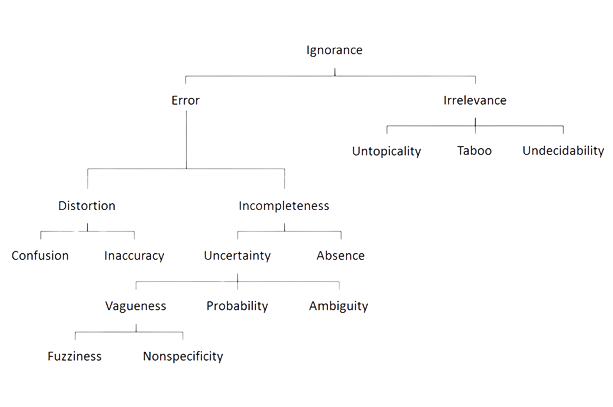
\includegraphics[width=0.75\linewidth]{images/smithson.png}
        \caption{Smithson's taxonomy of ignorance and uncertainty}
    \end{figure}
    To model ignorance, it is often decided to associate measures of certain aspects. Let's distinguish between two aspects:
    \begin{itemize}
        \item The type of representation: numbers, labels, intervals, etc.
        \item The represented ignorance that we would like to model, such as probability, reliability, subjective evaluation, etc.
    \end{itemize}
    Probability is represented with numbers between zero and one, and a well-established set of rules and properties are associated with its management. For example:
    \begin{itemize}
        \item The sum of probabilities should equal one.
        \item The probability a posteriori of a hypothesis $h_i$ given some evidence $e$ is given by the Bayes theorem:
            \[\textnormal{P}(h_i \mid e)=\dfrac{\textnormal{P}(e \mid h_i)\textnormal{P}(h_i)}{\textnormal{P}(e)}\]
    \end{itemize}

    Probability has been used in applications like MYCIN, one of the first expert systems designed for diagnosing blood illnesses. 
    MYCIN modeled certainty by considering two numerical factors:
    \begin{itemize}
        \item Measure of increased Belief: 
            \[\textnormal{MB}=\dfrac{\textnormal{P}\left(\dfrac{h}{e}\right)-\textnormal{P}(h)}{1-\textnormal{P}(h)}\]
        \item Measure of decreased Disbelief: 
            \[\textnormal{MD}=\dfrac{\textnormal{P}(h)-\textnormal{P}\left(\dfrac{h}{e}\right)}{\textnormal{P}(h)}\]
    \end{itemize}
    The measure of a statement is given by the certainty factor:
    \[\textnormal{CF}=\textnormal{MB}-\textnormal{MD} \in [-1;1]\]
    
    A key hypothesis for this solution is that the numbers given as $\textnormal{MB}$ and $\textnormal{MD}$ are not statistical probabilities but subjective probabilities, provided by different experts and combined using rules (which can introduce ambiguity).
    
    In comparison to probabilities, linguistic terms are less ambiguous than numbers. 
    Using a limited set of labels, it is possible to associate subjective evaluations with statements, making it relatively easy to achieve consensus on subjective judgments. 
    A computational mechanism is then needed to define how to combine labels. 
    This is achieved through the use of fuzzy systems, which represent the truth of a statement in linguistic terms and evaluate its fuzziness.
    
    \newpage

    \chapter{Fuzzy sets}
    \section{History}
    Fuzzy sets were introduced by Lotfi Zadeh in 1965 as a tool to model approximate concepts. 
    In 1972, the first linguistic fuzzy controllers were implemented. 
    By around 1980, fuzzy sets began to see frequent use worldwide. 
    In the 1990s, there was a massive proliferation of fuzzy controllers in various end-user goods. 
    Today, fuzzy systems form the core of many intelligent devices.

    \section{Fuzzy membership function}
    A crisp set is defined by a boolean membership function on some property of the considered elements. 
    In contrast, a fuzzy set is a set whose membership function ranges between zero and one.
    \begin{definition}
        A \emph{membership function} defines a set by specifying the degree of membership of an element from the universe of discourse to the set. 
        A \emph{label} is assigned to the set to provide a reference. 
        Fuzzy sets can also be defined with a variable having discrete values.
    \end{definition}
    \begin{figure}[H]
        \centering
        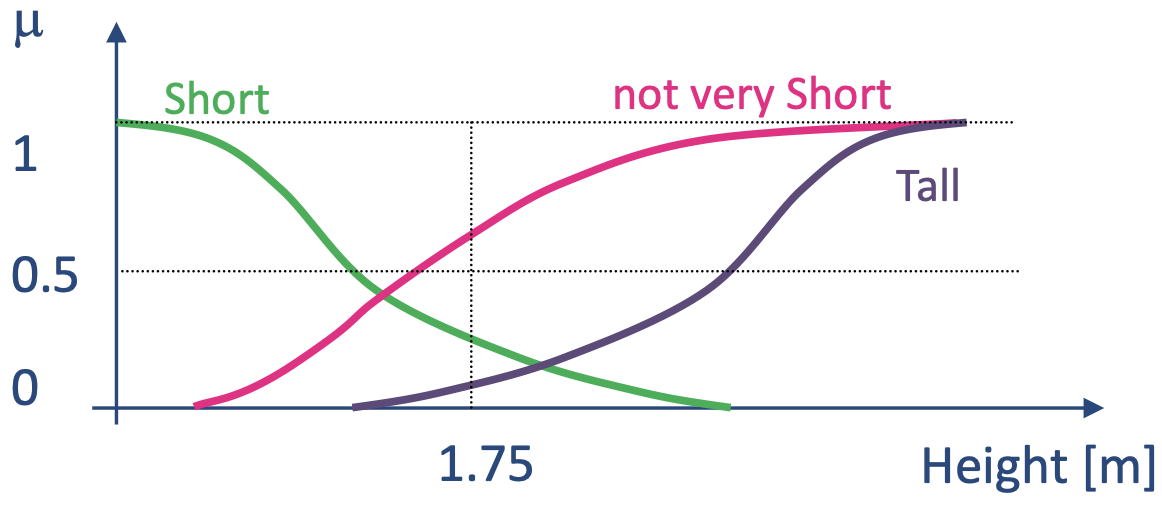
\includegraphics[width=0.4\linewidth]{images/function.png}
        \caption{Example of a membership function}
    \end{figure}
    To define a membership function, we need to consider the following steps based on the purpose of the model and the available data:
    \begin{enumerate}
        \item Select a variable on which the membership function will be defined.
        \item Define the range of the variable.
        \item Identify the fuzzy sets needed for the application and define the labels.
        \item Identify characteristic points for the membership function for each fuzzy set.
        \item Define the shape of the membership function.
        \item Verify the correctness of the membership function.
    \end{enumerate}
    The shapes of the membership function can be chosen arbitrarily. 
    The choice of shape affects the smoothness of the transition between two labels (e.g., a horizontal shape results in an immediate transition within intervals).
    \begin{figure}[H]
        \centering
        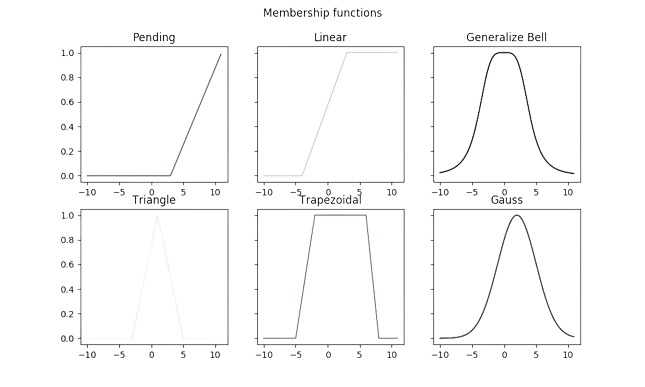
\includegraphics[width=0.75\linewidth]{images/shape.png}
        \caption{Possible shapes for a membership function}
    \end{figure}
    \begin{definition}
        A set of fuzzy sets that fully covers the universe of discourse is called a \emph{frame of cognition}. It has the following properties:
        \begin{itemize}
            \item Coverage: each element of the universe of discourse is assigned to at least one granule with membership greater than or equal to zero.
            \item Uni-modality of fuzzy sets: there is a unique set of values for each granule with maximum membership. 
        \end{itemize}

        A frame of cognition for which the sum of the membership values of each value of the base variable is equal to one is called a \emph{fuzzy partition}.

        The \emph{$\alpha$-cut} of a fuzzy set is the crisp set of values of $x$ such that $\mu(x) \geq \alpha$:
        \[\alpha_\mu(x)=\{x \mid \mu(x) \geq \alpha\}\]
    \end{definition}
    \begin{figure}[H]
        \centering
        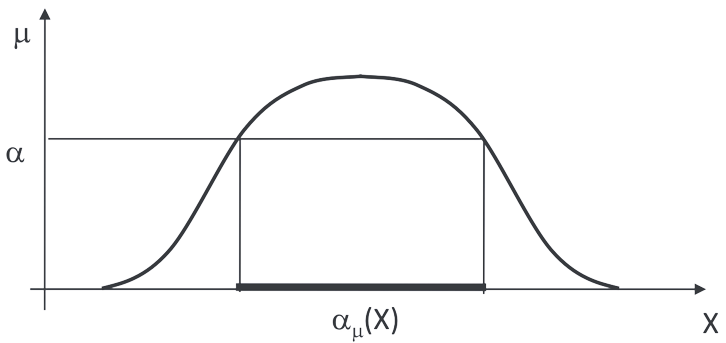
\includegraphics[width=0.4\linewidth]{images/alpha.png}
        \caption{Alpha-cut of a membership function}
    \end{figure}
    \begin{definition}
        The \emph{support} of a fuzzy set is the crisp set of values $x$ such that $\mu_f(x)>0$. 
    \end{definition}
    \begin{figure}[H]
        \centering
        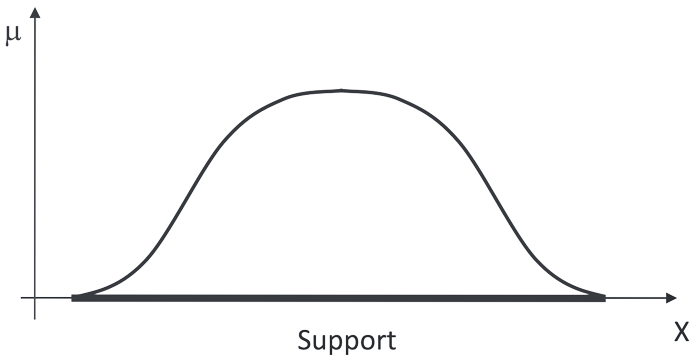
\includegraphics[width=0.4\linewidth]{images/support.png}
        \caption{Support of a membership function}
    \end{figure}
    \begin{definition}
        The height $h_f$ of a fuzzy set $f$ on the universe $X$ is the highest membership degree of an element of $X$ in the fuzzy set:
        \[h_f(X)=\max_{x \in X}\mu_f(x)\]
        A fuzzy set is considered normal if, and only if, $h_f(X)=1$.
    \end{definition}
    \begin{figure}[H]
        \centering
        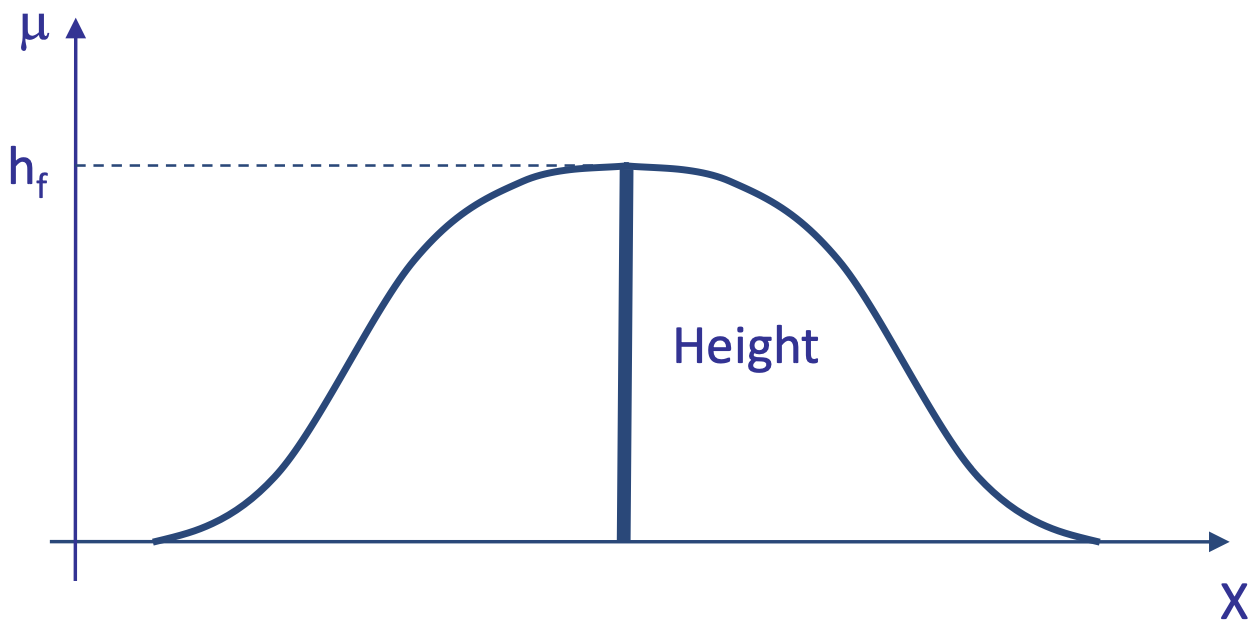
\includegraphics[width=0.4\linewidth]{images/height.png}
        \caption{Height of a membership function}
    \end{figure}
    \begin{definition}
        A fuzzy set is \emph{convex} if and only if 
        \[\mu[\lambda x_1+(1-\lambda)x_2] \geq \min [\mu(x_1),\mu(x_2)]\]
        for any $(x_1,x_2) \in \mathbb{R}$ and any $\lambda \in [0,1]$.
    \end{definition}
    \begin{figure}[H]
        \centering
        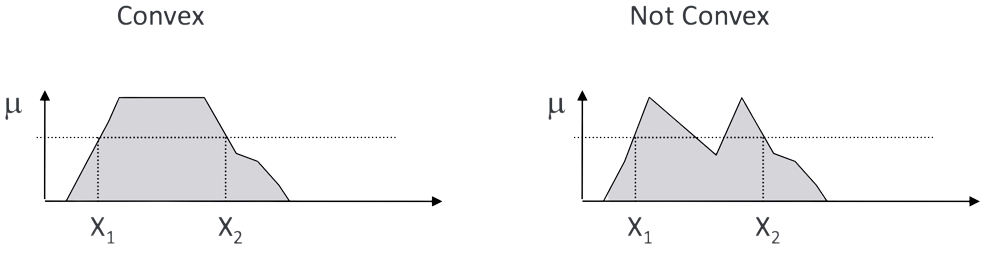
\includegraphics[width=0.75\linewidth]{images/convex.png}
        \caption{Graphical difference between a convex and a not convex set}
    \end{figure}
    The specific fuzzy sets include "singleton" (a fuzzy set comprising exactly one member) and "interval" (a fuzzy set where all members have a membership value equal to one). 
    The available operations on fuzzy sets encompass:
    \begin{itemize}
        \item Complement: $\mu_{\bar{f}}(x)=1-\mu_f(x)$.
        \item Union: $\mu_{f_1 \cup f_2}(x)=\max [\mu_{f_1}(x),\mu_{f_2}(x)]$.
        \item Intersection: $\mu_{f_1 \cap f_2}(x)=\min [\mu_{f_1}(x),\mu_{f_2}(x)]$.
    \end{itemize}

    \newpage

    \chapter{Fuzzy logic}
    \section{Introduction}
    Logic is a tool that has been employed for thousands of years to formally represent knowledge. There are various types of logic, including:
    \begin{itemize}
        \item Propositional logic: assigning truth values to propositions.
        \item First-order logic: assigning truth values to predicates, involving variables and quantifiers.
        \item Second-order logic: dealing with predicates of predicates.
    \end{itemize}
    These types of logic operate in a binary fashion. 
    It's worth noting that the specific meanings of terms within these logics are not inherently defined within the formalism itself, and such definitions are not necessary for the logic to function effectively.

    \section{Propositional logic}
    Propositional logics revolve around propositional operators that can be applied to one or more propositions to generate new propositions. 
    The primary focus lies on the truth value of propositions and how these truth values are combined.
    \begin{definition}
        A logic is considered \emph{truth functional} if the truth value of a compound sentence depends solely on the truth values of the individual atomic sentences, without regard to their meaning or structure. 
        For such a logic, the critical question regarding propositions is the range of truth values they may assume.
    \end{definition}
    In classical, Boolean, or two-valued logic, each proposition is either true or false, and no other characteristic of the proposition is considered relevant.
    The fundamental operators in propositional logics include conjunction ($\land$), disjunction ($\lor$), and negation ($\lnot$).

    \section{First order predicate logic}
    First-order logic extends propositional logic by introducing the capability to define predicates involving variables. 
    It also introduces the existential ($\exists$) and universal ($\forall$) quantifiers.
    In predicate logics, it is possible to deduce the truth value of a proposition through inferential mechanisms, such as Modus Ponens.
    \begin{example}
        Given the sentences: "All man are mortal" and "Socrates is a man" we can infer that "Socrates is mortal".
    \end{example}
    Inference is employed to model a mental mechanism that allows us to store a reduced amount of information and establish a process for deriving additional information from existing information to deal with everyday situations.
    \begin{definition}
        The combination of information and potential relationships constitutes what we refer to as \emph{knowledge}.
    \end{definition}

    \section{Many-valued logics}
    Aristotle raised questions about the suitability of classical logic as a knowledge representation tool.
    For example, classical logic struggles to determine the truth value of a proposition in the context of the future.
    To address this, a third value (e.g., 0.5) can be introduced to represent undefined situations, leading to the concept of three-valued logic. 
    This concept can be extended to infinite-value logics that consider a continuum of truth values between zero and one.

    \begin{example}[Logic L1, Łukasiewicz(1930)]
        In this type of infinite-value logic, the main rules include:
        \begin{itemize}
            \item $\textnormal{T}(\lnot a)=1-\textnormal{T}(a)$.
            \item $\textnormal{T}(a \land b)=\min (\textnormal{T}(a),\textnormal{T}(b))$.
            \item $\textnormal{T}(a \lor b)=\max (\textnormal{T}(a),\textnormal{T}(b))$.
            \item $\textnormal{T}(a \implies b)=\min (1, 1+\textnormal{T}(b)-\textnormal{T}(a))$.
            \item $\textnormal{T}(a \Leftrightarrow b)=1-\left\lvert \textnormal{T}(a)-\textnormal{T}(b) \right\rvert$.
        \end{itemize}
    \end{example}
    These innovations brought about a shift in society, where things are no longer categorically stated as true or false. 
    Probability (Kolmogorov, 1929) and stochasticity (Markov, 1906) became the preferred ways to represent this new approach to science and life.

    The differences between classical logic (L2) and many-valued logic (L1) include:
    \begin{itemize}
        \item L1 being isomorphic to fuzzy set theory, with standard operators, while classical logic L2 is isomorphic to set theory.
        \item Tautologies, which are true by definition and used to prove theorems in classical logic L2, may not be valid in L1. 
            For example, the third excluded law ($\textnormal{T}(a \lor \lnot a)=1$) and the non-contradiction law ($\textnormal{T}(a \land \lnot a)=0$) are not valid in L1.
    \end{itemize}
    In classical logic, the sentence "I'm a liar" would be considered a paradox if we assign meaning to the term "liar," as no formula can have the same truth value as its negation. 
    However, this may not be the case in many-valued logics. In Łukasiewicz logic, for instance, it's possible for a sentence to have a truth value of 0.5, and its negation to also have a truth value of 0.5, making the proposition consistent with the axioms and not a paradox.

    \section{Fuzzy logic}
    Fuzzy logic is an infinite-valued logic with truth values ranging from 0 to 1, where propositions are expressed in the form of "A is L," where:
    \begin{itemize}
        \item A is a linguistic variable.
        \item L is a label representing a fuzzy set.
    \end{itemize}
    Formally, a linguistic variable is defined by a 5-tuple (X, T(X), U, G, M), where: 
    \begin{itemize}
        \item X is the name of the variable.
        \item T(X) is the set of term for X, each corresponding to a fuzzy variable denoted by T(X) and ranging on U.
        \item U is the universe of discourse defined on a base variable u.
        \item G is the syntactic rule used to generate the interpretation X of each value u.
        \item M is the semantic rule used to associate to X its meaning.
    \end{itemize}
    \begin{example}
        Let's define a linguistic variable for age as follows:
        \begin{itemize}
            \item X is a linguistic variable labelled "age".
            \item $\textnormal{U}=[0,100]$.
            \item $\textnormal{T(X)}=\{old, middle-aged, young, \dots\}$.
            \item $\textnormal{u}=[0,+\infty]$.
            \item M represents the definition in terms of fuzzy sets for the values of X.
            \item G is responsible for the fuzzy matching interpretation of u.
        \end{itemize}
    \end{example}
    Now that we have defined the linguistic variable, it is possible to express a simple proposition as "p: X is F", where:
    \begin{itemize}
        \item X is a linguistic variable.
        \item F is the label of a fuzzy set defined on U, representing a fuzzy predicate.
        \item $\mu_{\textnormal{F(x)}}$ is the membership function defining F, and it is interpreted as the truth value for the proposition p ($\textnormal{T(p)}=\mu_{\textnormal{F(x)}}$).
    \end{itemize}
    Hence, the truth value of the proposition P is a fuzzy set defined on the interval $[0,1]$.
    \begin{example}
        Consider the simple proposition "p: temperature is high", with X representing temperature and F representing high. 
        We can determine the truth value of this proposition using the graph of the membership function as shown below:        
        \begin{figure}[H]
            \centering
            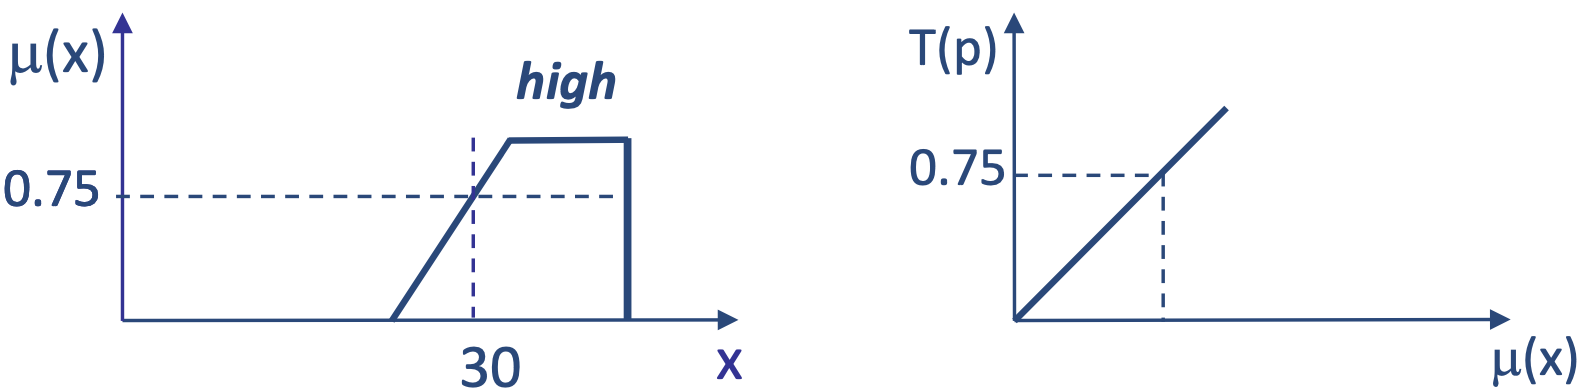
\includegraphics[width=0.5\linewidth]{images/temperature.png}
        \end{figure}
        Consequently, the truth value of the given proposition is 0.75.
    \end{example}

    It is also possible to express qualified, non-conditional propositions using the syntax "p: (X is F) is S", where:
    \begin{itemize}
        \item S is a fuzzy truth qualifier.
        \item F is a fuzzy set.
        \item p is truth qualified.
    \end{itemize}
    \begin{example}
        Consider the conditional proposition "p: age of Tina is young is very true", where X represents age, F represents young, and S represents very true. 
        To determine the truth value of this proposition, we can refer to the graph of the membership function as shown below:
        \begin{figure}[H]
            \centering
            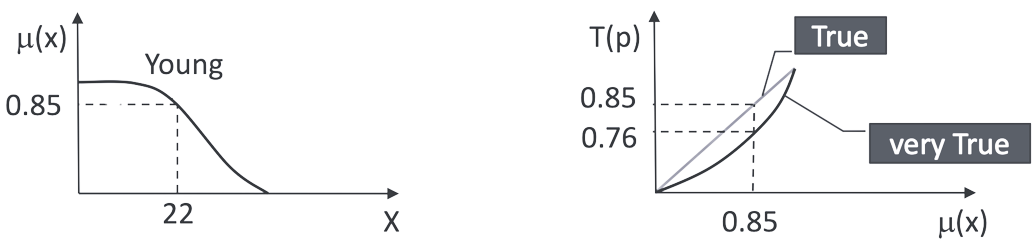
\includegraphics[width=0.75\linewidth]{images/age.png}
        \end{figure}
    \end{example}

    In fuzzy logic, fuzzy modifiers are employed to adjust the truth values of propositions. These modifiers can be categorized into two main types:
    \begin{itemize}
        \item Strong ($m(a) \leq a \: \forall a \in [0 \dots 1]$): these modifiers strengthen the predicate, leading to a reduction in the truth value of the proposition.
        \item Weak($m(a) \geq a \: \forall a \in [0 \dots 1]$): these modifiers weaken the predicate, resulting in an increase in the truth value of the proposition.
    \end{itemize}
    The key properties of fuzzy modifiers include:
    \begin{itemize}
        \item $m(0)=0$ and $m(1)=1$.
        \item $m$ is a continuous function. 
        \item If $m$ is a strong modifier, then $m^{-1}$ is a weak modifier, and vice versa.
        \item When combining another modifier $g$ with $m,$ and vice versa, the resulting composition is also a modifier. 
            If both $m$ and $g$ are strong (or weak), their composition is also strong (or weak).
    \end{itemize}
    \begin{example}
        The sentence "x is young" can be represented as "(x is young) is true". This sentence can be modified using fuzzy modifiers in the following ways:
        \begin{itemize}
            \item x is very young is true.
            \item x is young is very true.
            \item x is very young is very true.
        \end{itemize}
        Graphically, we can visualize the modified membership function as follows:
        \begin{figure}[H]
            \centering
            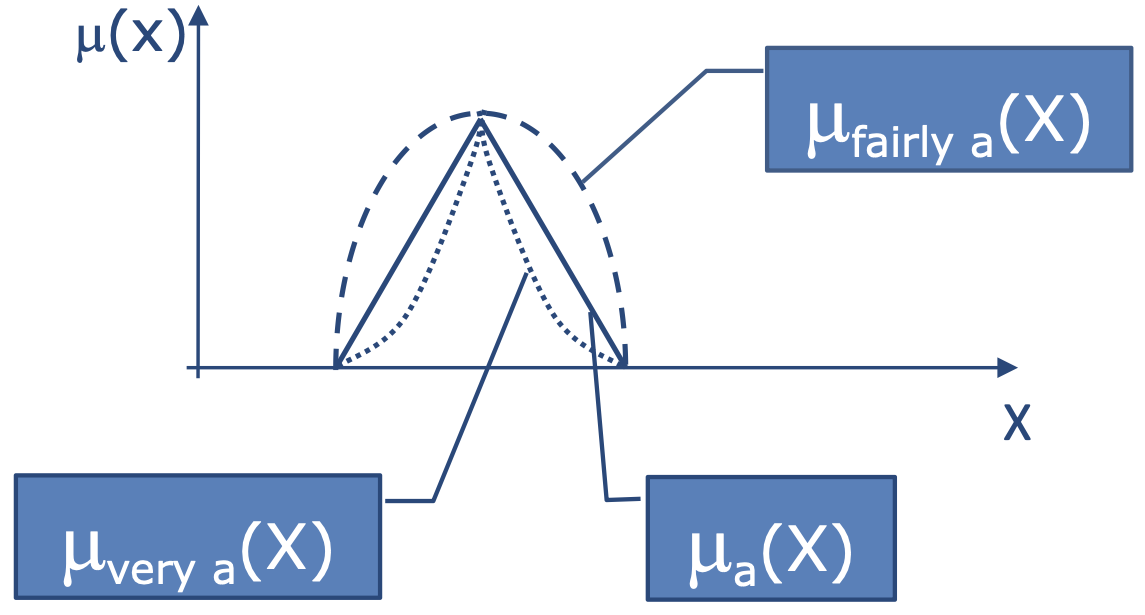
\includegraphics[width=0.4\linewidth]{images/modifiers.png}
        \end{figure}
        Here, we have:
        \begin{itemize}
            \item $\mu_{very \: a}(x)=\mu_a(x)^2$.
            \item $\mu_{fairly \: a}(x)=\mu_a(x)^{\dfrac{1}{2}}$.
        \end{itemize}
    \end{example}

    \section{Inference rules}
    \begin{definition}
        An \emph{inference rule} is a model, essentially defining a mapping from input to output. 
        These rules are utilized to represent inferential relationships among various pieces of knowledge.
    \end{definition}
    We will primarily focus on forward chaining rules, which typically have the structure "IF antecedent THEN consequent", where: 
    \begin{itemize}
        \item antecedent is a set of clauses related by logical operators.
        \item consequent is a set of clauses related by logical operators.
    \end{itemize}
    In these inference rules, the clauses can be either propositions (sequences of symbols) or patterns (sequences of symbols and variables).

    Inference rules play a crucial role in the implementation of Knowledge-Based Systems, with Expert Systems standing out as highly successful applications in the field of Artificial Intelligence. 
    Expert Systems are carefully designed to replicate or enhance human expertise in problem-solving. 
    The process of Knowledge Acquisition, which is inherently intricate, leads to the development of rule-based systems that are executed on computer platforms.
    A system can generate new information by following these steps:
    \begin{enumerate}
        \item Pattern matching: identify the rules with antecedents that match the known facts stored in the fact base. 
            These rules can be considered for activation, provided the corresponding variables are assigned.
        \item Rule selection: among the rules identified through pattern matching (candidate rules), select the ones to be activated.
        \item Rule activation: assert the consequents of the selected rules in the fact base.
    \end{enumerate}
    \begin{example}
        Let's consider a rule base consisting of the following four rules:
        \begin{enumerate}
            \item IF X croaks AND X eats flies, THEN X is a frog.
            \item IF X chirps AND X sings, THEN X is a canary.
            \item IF X is a frog, THEN X is green.
            \item IF X is a canary, THEN X is yellow.
        \end{enumerate}
        Now, let's observe the following facts in the fact base:
        \begin{itemize}
            \item Fritz croaks.
            \item Fritz eats flies.
        \end{itemize}
        From rule 1 and the facts (a and b), we can add the following fact to the fact base:
        \[\textnormal{Fritz is a frog}\]
        With the updated fact base, we can use rule 3 to deduce the fact:
        \[\textnormal{Fritz is green}\]
    \end{example}

    \section{Fuzzy rules}
    \begin{definition}
        A \emph{fuzzy rule} is a rule whose clauses have the form "V is L", where V is a linguistic variable, and L is a label representing a value for V associated with a fuzzy set.
        Each of these clauses is referred to as a \emph{linguistic clause}. 
    \end{definition}
    Often, clauses in the antecedent are implicitly connected by the AND operator, which is not explicitly written.
    The antecedent is typically compared to facts represented as values of base variables corresponding to the linguistic variables. 
    The consequent can be one of two types:
    \begin{itemize}
        \item Linguistic rules: the consequent is a conjunction of linguistic clauses. 
            These rules can be viewed as a mapping between the interpretation of an input configuration and a symbolic description of the desired output. 
            The general formula is:
            \[\textnormal{IF }(\textnormal{A is }L_{A_i})\textnormal{ AND }(\textnormal{B is }L_{B_k})\textnormal{ AND }\dots\textnormal{ THEN }(\textnormal{U is }L_{U_m})\textnormal{ AND }\dots\]
        \item Model rules: associate a model with the linguistic interpretation of its applicability conditions. 
            This can be seen as a mapping between the interpretation of an input configuration and a model that is applied to the input real values to obtain the output. 
            The general formula is:
            \[\textnormal{IF }(\textnormal{A is }L_{A_n})\textnormal{ AND }(\textnormal{B is }L_{B_k})\textnormal{ AND }\dots\textnormal{ THEN } \textnormal{U is } f(\textnormal{A,B})\]
    \end{itemize}
    The steps for using fuzzy rules are as follows:
    \begin{enumerate}
        \item Input matching.
        \item Combining matching degrees.
        \item Combining with rule weight, if present.
        \item Aggregating output from different rules.
        \item Optionally, defuzzification of the output.
    \end{enumerate}

    When defuzzifying the output, various operators can be considered in addition to the weighted mean. 
    These operators include the centroid, bisector, average of maxima, the lowest maximum, the highest maximum, center of the highest area, and more. 
    The choice of operator can impact the system's output and the level of optimization.
    \begin{example}
        Let's consider the following scenario:
        \begin{itemize}
            \item Two input variables, A and B, each with fuzzy partitions distributed equally from Negative Large to Positive Large.
            \item One output variable U (equally distributed fuzzy set) from Negative Large to Positive Large. The fuzzy sets are all singletons.
        \end{itemize} 
        \begin{figure}[H]
            \centering
            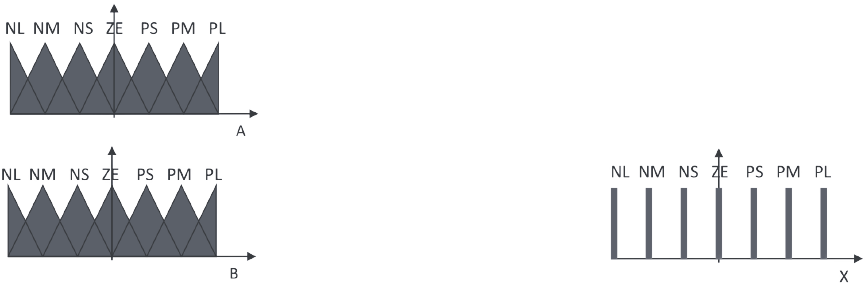
\includegraphics[width=0.5\linewidth]{images/rules.png}
        \end{figure}
        To define the rules of the rule base, along with their weights, we have the following rules:
        \begin{enumerate}
            \item IF A is $PL$ AND B is $PS$ THEN X is $PM$ (weight 1).
            \item IF A is $PM$ AND B is $PS$ THEN X is $PS$ (weight 0.5).
            \item IF A is $PL$ AND B is $PM$ THEN X is $PM$ (weight 1).
        \end{enumerate}
        Now, let's set A to 22 and B to 140. 
        The steps used to calculate the output value are as follows:
        \begin{enumerate}
            \item For the first step, we need to check the corresponding truth value for each label:
                \begin{itemize}
                    \item (A is $PL$) has a truth value of 0.2.
                    \item (B is $PS$) has a truth value of 0.6.
                    \item (A is $PM$) has a truth value of 0.8.
                    \item (B is $PM$) has a truth value of 0.4.
                \end{itemize}
            \item To consider the degree of truth of each predicate, we simply take the minimum between the two values (due to the AND operator). 
                Thus, we get: 
                \begin{itemize}
                    \item 0.2 for the first rule. 
                    \item 0.6 for the second. 
                    \item 0.4 for the third.
                \end{itemize}
            \item Now we have to consider the rule weight. 
                To do this, we select the minimum between the previously calculated value and the weight value. 
                So, the final values for the consequents are as follows:
                \begin{itemize}
                    \item 0.2 for the first rule. 
                    \item 0.5 for the second. 
                    \item 0.4 for the third.
                \end{itemize}
            \item To aggregate the output, we take the maximum value when we have a repeated expression. 
                In this case, we obtain that: 
                \begin{itemize}
                    \item (X is $PM$) has a truth value of 0.4.
                    \item (X is $PS$) has a truth value of 0.5.
                \end{itemize}
                This result can be visualized graphically by cutting the initial graph: 
                \begin{figure}[H]
                    \centering
                    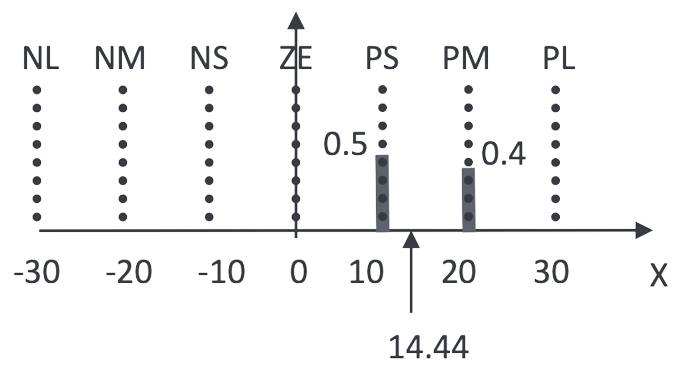
\includegraphics[width=0.4\linewidth]{images/cut.png}
                \end{figure}
            \item Finally, to defuzzify the result and obtain a numerical value, we can use a simple weighted mean:
                \[\textnormal{U}=\dfrac{10 \cdot 0.5 + 20 \cdot 0.4}{0.5+0.4}=14.44\]
        \end{enumerate}
    \end{example}
    \begin{example}
        Consider the same variables as in the previous example. This time, we are using different rules:
        \begin{enumerate}
            \item IF A is $PL$ and B is $PS$ THEN X is $A+2B$.
            \item IF A is $PM$ and B is $PS$ THEN X is $A+3$. 
            \item IF A is $PL$ and B is $PM$ THEN X is $A+B$.
        \end{enumerate}
        All the models used in these rules are linear. 
        Pattern matching is the same as in the previous example, leading to the following degree of truth for the rules: the first one has a value of 0.2, the second has a value of 0.5, and the third has a value of 0.4.
        For the output aggregation, we again use the weighted mean and apply it to the initial values of $A=22$ and $B=140$:
        \[\textnormal{U}=\dfrac{0.2 \cdot (A+2B)+0.5 \cdot (A+3)+ 0.4 \cdot (A+B)}{0.2+0.5+0.4}=125.18\]
    \end{example}

    \section{Fuzzy system design}
    The structured approach to develop a fuzzy system for solving specific problems consist of: 
    \begin{enumerate}
        \item Problem definition.
        \item Parametrization of the model: concepts.
        \item Mapping definition: rules.
        \item Implementation.
        \item Testing.
    \end{enumerate}
    In the problem definition phase of designing a fuzzy system, it's essential to choose the input and output variables and clearly define the goal of the model. 
    Input variables are typically numerical or ordinal variables, making it possible to define fuzzy sets on them. 
    These variables can be categorized as follows:

    \begin{itemize}
        \item Perceived values: these variables come directly from sensors, collected data, or user inputs.
        \item Computed variables: these are derived from perceived variables through calculations or processing.
    \end{itemize}
    The choice of input variables is a design decision, and there aren't inherently best or worst input variables to select. 
    Output variables, on the other hand, depend on the specific needs of the modeler and are the result of the fuzzy model's computations. 
    The goals of the fuzzy model should be defined in advance and should guide the design process.

    During the system parametrization phase, several key decisions need to be made:
    \begin{itemize}
        \item Selection of membership functions: this involves choosing appropriate membership functions for all variables. 
            Membership functions can be defined by a single expert based on objective evaluation or interviews, by multiple experts for increased reliability, or even by automatic systems working on data (e.g., using Neural Networks). 
            The number of membership functions for each variable typically ranges from three to seven. 
            It's important to ensure that every point within the range of input variables is covered by at least one fuzzy set that participates in at least one rule. 
            The boundaries should be covered with the maximum value to avoid any gaps in coverage.
        \item Selection of inferential mechanism: the inferential engine depends on the operators selected for different parts of the rule-based system:
            \begin{itemize}
                \item AND of antecedent clauses: the choice between using the minimum (where the worst degree of matching is the most relevant) or the product (where all degrees of matching are relevant).
                \item Detachment: this involves combining the degree of truth with the rule weight. 
                    You can choose between using the minimum or the product.
                \item Aggregation of degrees of the same consequent: you can choose between using the maximum (where the best degree is the most relevant) or the probabilistic sum (where all knowledge is considered).
            \end{itemize}
        \item Selection of fuzzification and defuzzification: this step involves deciding whether to apply fuzzification (converting crisp input values into fuzzy values) and defuzzification (converting fuzzy output values back into crisp values) in your system.
    \end{itemize}
    These decisions are crucial to the performance and behavior of your fuzzy system and should align with the goals and requirements defined in the problem definition phase.
    The design and definition of fuzzy rules can be carried out using various approaches, and the testing phase helps ensure the effectiveness and reliability of the system. Here are some methods for rule definition: 
    \begin{itemize}
        \item From experience: rules can be formulated based on the domain knowledge and expertise of human operators or experts who understand the system. 
            hese rules are often based on their experience and intuition.
        \item From another model: in some cases, existing models, such as mathematical models or traditional control systems, can be used as a basis for defining fuzzy rules.
            These models can be adapted into fuzzy rule sets.
        \item Machine Learning: Machine learning techniques, including supervised learning methods, can be used to derive fuzzy rules from data. 
            Algorithms like decision trees, genetic algorithms, or neural networks can automatically generate fuzzy rule sets from training data.
        \item Self-tuning techniques: some systems employ self-tuning mechanisms, like Neural Networks or reinforcement learning algorithms, to adapt and modify fuzzy rules based on ongoing system feedback. 
            These methods can optimize rule sets over time.
    \end{itemize}
    Testing can be conducted using:
    \begin{itemize}
        \item Dynamic simulation: dynamic simulation involves running the fuzzy system in a simulation environment to assess its performance under various conditions and scenarios. 
            This allows for a thorough evaluation of how the system responds to different inputs and situations.
        \item Static simulation: static simulation involves testing the fuzzy system with predefined inputs and observing its outputs. 
            This can help evaluate the system's consistency and ensure that it adheres to expected behavior without the need for a real-time dynamic simulation.
        \item Direct testing on the process: in some cases, fuzzy systems can be tested directly on the real process, typically under safe or controlled conditions. 
            This testing approach validates the system's performance in the actual operational environment, which is valuable for systems that control physical processes.
    \end{itemize}
    The choice of rule definition and testing methods depends on the specific application, available data, and the complexity of the system. 
    Additionally, it's essential to validate and refine the fuzzy rule set to achieve the desired system behavior and performance.

    \section{Applications of fuzzy systems}
    Fuzzy control systems are designed to regulate the behavior of other systems, often employing a PID controller where the output relies on the disparity between the desired and observed behavior. 
    The general structure of a fuzzy control system is illustrated in the figure below:
    \begin{figure}[H]
        \centering
        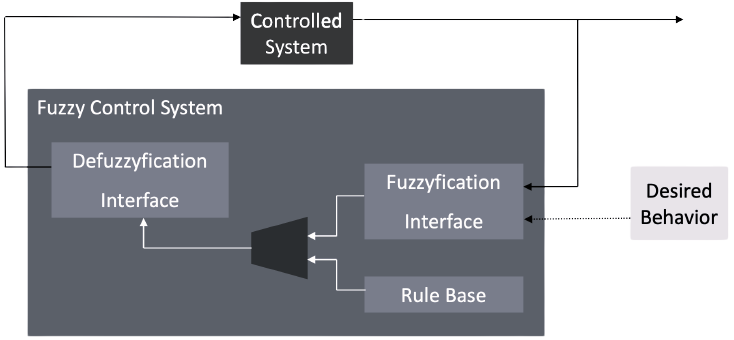
\includegraphics[width=0.5\linewidth]{images/control.png}
    \end{figure}
    Key attributes of a fuzzy control system include:
    \begin{itemize}
        \item Robustness in the presence of noise.
        \item Control rules applicable over a broad range.
        \item Capability to model expert heuristics.
        \item Smooth action.
        \item Inherent non-linearity.
    \end{itemize}
    Additionally, fuzzy systems have the potential to facilitate flexible, human-like database queries. 
    For instance, fuzzy sets can be employed to formulate queries such as "Provide the names of individuals who have recently made substantial investments", thereby imbuing "recently" and "a lot" with meaningful interpretations.

    Fuzzy systems find applications in various domains within Artificial Intelligence, including Expert Systems, scheduling, and Decision Support Systems.

    \newpage

    \chapter{Evidence theory}
    \section{Fuzzy mathematics}
    Fuzzy numbers are a mathematical concept used to model our perception of approximate values. 
    They are essentially fuzzy sets defined over the set of real numbers. 
    Three important constraints are used to define fuzzy numbers:
    \begin{enumerate}
        \item Normal fuzzy sets: fuzzy numbers adhere to the principles of normal fuzzy sets, which allows them to capture the concept of approximate value.
        \item Convex fuzzy sets: for a fuzzy number to be well-defined, all $\alpha$-cut intervals should be closed. This is a key constraint for arithmetic operations.
        \item Bounded support: the support of a fuzzy number (the range where it has significant membership) should be bounded, providing further constraints for their definition.
    \end{enumerate}
    Fuzzy sets can be used to define various types of numerical representations, including fuzzy numbers, fuzzy intervals, defined intervals, and crisp numbers, as illustrated in the provided figure.
    \begin{figure}[H]
        \centering
        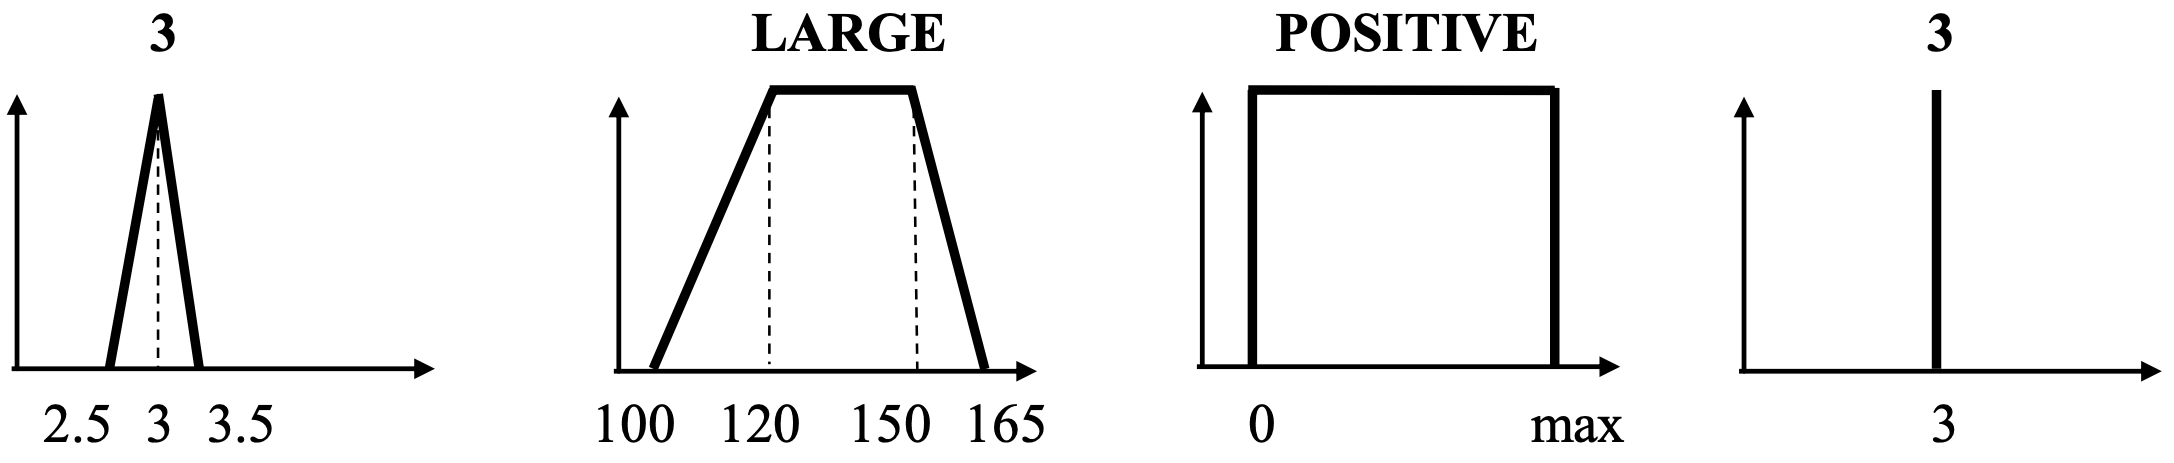
\includegraphics[width=0.75\linewidth]{images/numbers.png}
        \caption{Possible representation of numbers}.
    \end{figure}
    The arithmetic of fuzzy numbers is based on two primary properties:
    \begin{itemize}
        \item Uniqueness of $\alpha$-cuts: each fuzzy number can be fully represented by its $\alpha$-cuts, which are unique for that number.
        \item Closed intervals: the $\alpha$-cuts of fuzzy numbers are closed intervals of real numbers, which is crucial for arithmetic operations.
    \end{itemize}
    The four main arithmetic operators for fuzzy numbers are defined by combining operations on the intervals (represented by $\alpha$-cuts) that make up the fuzzy number:
    \begin{itemize}
        \item Addition: $[a,b]+[d,e]=[a+d,b+e]$.
        \item Subtraction: $[a,b]-[d,e]=[a-e,b-d]$.
        \item Multiplication:  $[a,b] \times [d,e]=[\min (ad,ae,bd,be),\max (ad,ae,bd,be)]$
        \item Division: $[a,b] \div [d,e]=\left[\min \left(\dfrac{a}{d},\dfrac{a}{e},\dfrac{b}{d},\dfrac{b}{e}\right),\max \left(\dfrac{a}{d},\dfrac{a}{e},\dfrac{b}{d},\dfrac{b}{e}\right)\right]$ with the condition that $[d,e] \neq [0,0]$ to avoid division by zero.
    \end{itemize}
    These operators allow for performing arithmetic operations on fuzzy numbers, taking into account the uncertainty or fuzziness associated with each value.
    \begin{example}
        Given the fuzzy numbers $[1,3]$ and $[4,6]$, we have the following operations:
        \begin{itemize}
            \item Addition of fuzzy numbers: the sum is calculated as the sum of the minimum and maximum values in each interval, resulting in 
            \[[1,3] + [4,6] = [1+4, 3+6] = [5,9]\]
            Graphically, this operation is represented as follows:
                \begin{figure}[H]
                    \centering
                    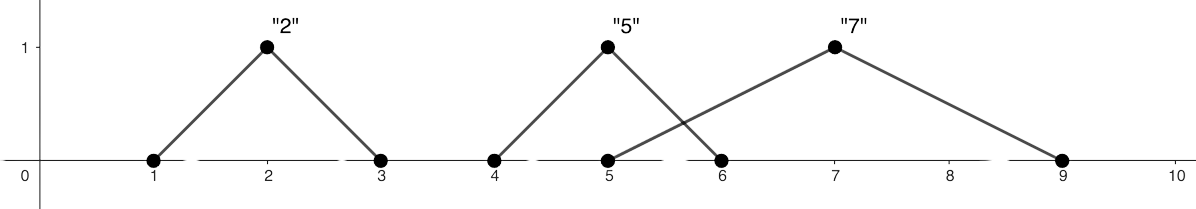
\includegraphics[width=0.75\linewidth]{images/sum.png}
                \end{figure}
            \item Subtraction of fuzzy numbers: the difference is found by subtracting the minimum of the first interval from the maximum of the second and subtracting the maximum of the first interval from the minimum of the second, yielding 
            \[[1,3] - [4,6] = [1-6, 3-4] = [-5,-1]\]
            Graphically, this operation is shown below:
                \begin{figure}[H]
                    \centering
                    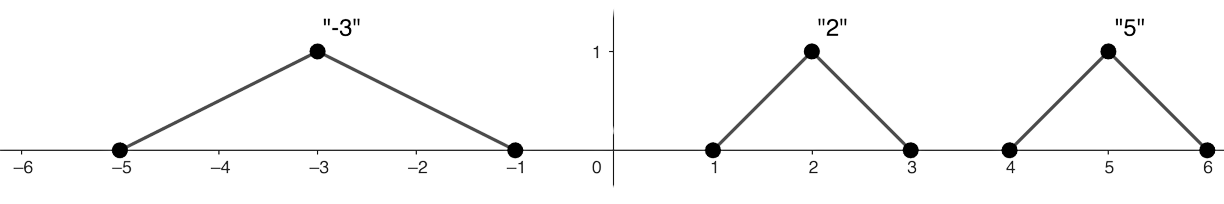
\includegraphics[width=0.75\linewidth]{images/subtraction.png}
                \end{figure}
            \item Multiplication of fuzzy numbers: the product is determined by taking the minimum and maximum values of the products of corresponding elements, resulting in 
            \[[1,3] \times [4,6] = [\min(1 \cdot 4, 1 \cdot 6, 3 \cdot 4, 3 \cdot 6), \max(1 \cdot 4, 1 \cdot 6, 3 \cdot 4, 3 \cdot 6)] = [4,18]\]
            Graphically, this operation is represented as follows:
                \begin{figure}[H]
                    \centering
                    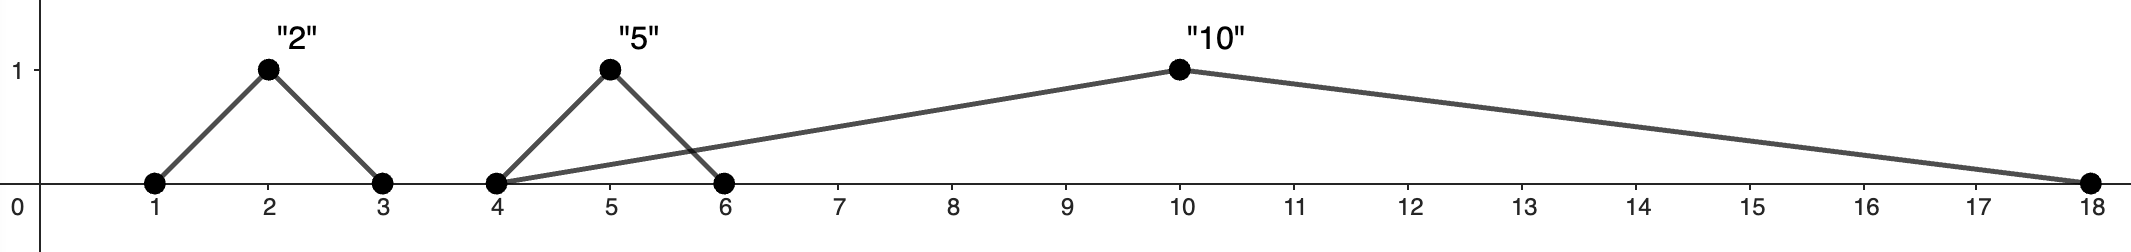
\includegraphics[width=0.75\linewidth]{images/multiplication.png}
                \end{figure}
            \item Division of fuzzy numbers: the division is obtained by finding the minimum and maximum values of the divisions of corresponding elements, leading to:
            \[[1,3] \times [4,6]=\left[\min\left(\dfrac{1}{4}, \dfrac{1}{6}, \dfrac{3}{4}, \dfrac{3}{6}\right),\max\left(\dfrac{1}{4}, \dfrac{1}{6}, \dfrac{3}{4}, \dfrac{3}{6}\right)\right]=\left[\dfrac{1}{6},\dfrac{3}{4}\right]\]
            Graphically, this operation is shown as follows:
                \begin{figure}[H]
                    \centering
                    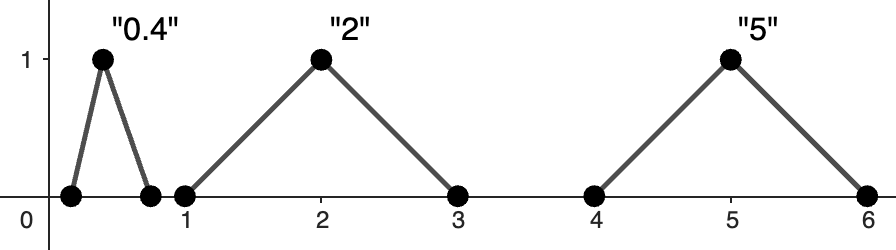
\includegraphics[width=0.5\linewidth]{images/division.png}
                \end{figure}
        \end{itemize}
    \end{example}
    From fuzzy arithmetic, it is also possible to define fuzzy functions, fuzzy integrals, and fuzzy derivatives. 
    In general, fuzzy numbers are employed to represent approximations.

    \section{Fuzzy measure and probability assignment}
    \begin{definition}
        A field is considered a \emph{Borel field} if it possesses the property that when all the $A_n$ sets belong to the field, the union and intersection of these sets also belong to the field. 
        A function $g$ defined on a Borel field B within the universe of discourse X is referred to as a \emph{fuzzy measure} if it satisfies the following properties:
        \begin{enumerate}
            \item $g(\varnothing)=0$ and $g(X)=1$.
            \item If $A,B \in B$ and $A \subseteq B$, then $g(A) \leq g(B)$.
            \item If $A_n \in B$ and $A_1 \subseteq A_2 \subseteq \dots$ then $\lim_{n \to \infty}g(A_n)=g\left(\lim_{n \to \infty}A_n\right)$.
        \end{enumerate}
    \end{definition}
    The concept of a fuzzy measure differs from a classical measure, as it relaxes the requirement of additivity.
    \begin{definition}
        The \emph{basic probabilistic assignment} is defined as follows:
        \begin{itemize}
            \item $m:\mathcal{P}(X) \rightarrow [0,1]$.
            \item $m(\varnothing)=0$.
            \item $\sum_{A \in \mathcal{P}(X)}m(A)=1$.
        \end{itemize}
        Here, $m$ provides, for any set A belonging to the power set of X$(\mathcal{P}(\textnormal{X}))$, an indication of how much the available and relevant evidence supports the notion that a given element belongs to set A.
    \end{definition}
    It's important to note that there is no requirement for $m(X)$ to be equal to 1, no necessity for $m(A) \leq m(B)$ when $A\subseteq B$, and no inherent relationship between $m(A)$ and $m(\lnot A)$.

    \section{Evidence theory}
    We aim to establish a measure of evidence for or against a proposition, employing two fuzzy measures: Belief and Plausibility.
    \begin{definition}
        \emph{Belief} is an estimate of the minimum probability that can be assigned to an element, considering the collected evidence. It is defined as follows:
        \begin{itemize}
            \item $Bel:\mathcal{P} (X) \rightarrow [0,1]$.
            \item $Bel(\varnothing)=0$ and $Bel(X)=1$.
            \item $Bel(A_1 \cup A_2 \cup \dots \cup A_n) \geq \sum_{j}Bel(A_j)-\sum_{j<k}Bel(A_j \cap A_k)+\dots+(-1)^{n+1}Bel(A_1 \cap A_2 \cap \dots \cap A_n)$
            \item $Bel(A)+Bel(\lnot A) \leq 1$.
        \end{itemize}

        \emph{Plausibility} is an estimate of the maximum probability that can be assigned to an element, considering the collected evidence. It is defined as follows:
        \begin{itemize}
            \item $Pl:\mathcal{P} (X) \rightarrow [0,1]$.
            \item $Pl(\varnothing)=0$ and $Pl(X)=1$.
            \item $Pl(A_1 \cap A_2 \cap \dots \cap A_n) \geq \sum_{j}Pl(A_j)-\sum_{j<k}Pl(A_j \cup A_k)+\dots+(-1)^{n+1}Pl(A_1 \cup A_2 \cup \dots \cup A_n)$
            \item $Pl(A)+Pl(\lnot A) \geq 1$.
        \end{itemize}
    \end{definition}
    Evidence theory finds application when multiple sources of knowledge exist, and the basic probability assignment is distributed across different sets of statements or intervals. 
    In such cases, we can utilize the characteristics of evidence theory to accumulate basic probability assignments and combine them to assess upper and lower bounds for the probability of a single statement. 
    Evidence theory implies
    \begin{itemize}
        \item There's no need to obtain a precise measurement from a knowledge source or experiment if it's not realistic or feasible.
        \item The principle of insufficient reason is not imposed. 
            Statements can be made about the likelihood of multiple events together without making assumptions about the probabilities of individual events under ignorance.
        \item The axiom of additivity is not imposed. 
            The measures can have the following properties:
            \begin{itemize}
                \item Add up to exactly one, which corresponds to a traditional probabilistic representation.
                \item Add up to less than one (sub-additive case), indicating incompatibility between multiple sources of information providing conflicting data.
                \item Add up to more than one (super-additive), suggesting a cooperative effect between multiple sources of information, such as multiple sensors providing the same information.
            \end{itemize}
    \end{itemize}
    
    Given five sources ($A, B, C, D, E$ with $A$ as the target) of information, four cases can arise:
    \begin{itemize}
        \item in this scenario, each source provides evidence for disjoint sets.
            \begin{figure}[H]
                \centering
                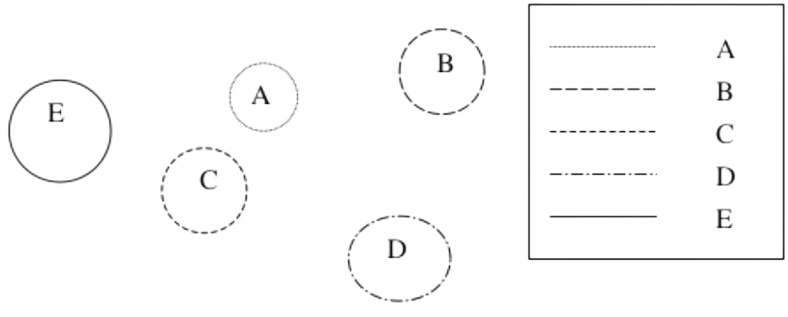
\includegraphics[width=0.5\linewidth]{images/conflict.png}
            \end{figure}
        \item Consonance: sources provide some evidence on nested sets, converging on the target.
            \begin{figure}[H]
                \centering
                
\includegraphics[width=0.5\linewidth]{images/consonance.png}
            \end{figure}
        \item Arbitrary: in the arbitrary case, each source provides evidence for sets, but only some of them include the target hypothesis.
            \begin{figure}[H]
                \centering
                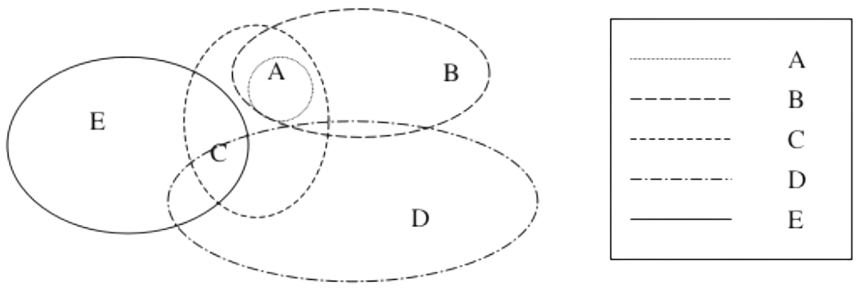
\includegraphics[width=0.5\linewidth]{images/arbitrary.png}
            \end{figure}
        \item Consistent: in this situation, all sources provide evidence for sets that include the same hypothesis.
            \begin{figure}[H]
                \centering
                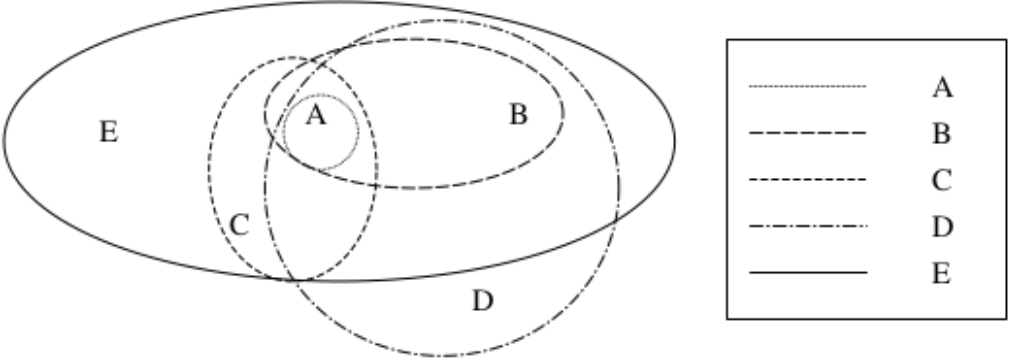
\includegraphics[width=0.5\linewidth]{images/consistent.png}
            \end{figure}
    \end{itemize}
    To combine the basic probability assignments, the Dempster rule of combination can be used:
    \[m_{1,2}(A)=\dfrac{\sum_{B \cap C=A}m_1(B)m_2(C)}{1-K}\]
    Where $K$ is the basic probability mass associated with conflict. 
    The role of $K$ in the denominator has the effect of completely ignoring conflict and attributing any probability mass associated with conflict to the null set. 
    The value of this variable is determined by:
    \[K=\sum_{B \cap C=O}m_1(B)m_2(C)\]
    \begin{example}
        Let's consider the discovery of an old painting strongly resembling paintings by Raphael. 
        This discovery raises various questions about the painting's status. 
        We have three questions:
        \begin{enumerate}
            \item Is the discovered painting a genuine painting by Raphael?
            \item Is the discovered painting a product of one of Raphael's many disciples?
            \item Is the discovered painting a counterfeit?
        \end{enumerate}
        Assume that two experts conducted careful examinations of the painting and provided us with basic assignments $m_1$ and $m_2$. 
        Using the introduced formulas, we can compute the plausibility and belief of all the subsets of hypotheses.
    \end{example}

    \section{Possibility and necessity}
    \begin{definition}
        \emph{Possibility} is another fuzzy measure that operates on sets. 
        
        A \emph{possibility measure} is represented by the function $\Pi : \mathcal{P}(X) \rightarrow [0,1]$, and it adheres to the following properties:
        \begin{enumerate}
            \item $\Pi(\varnothing)=0$ and $\Pi(X)=1$.
            \item $A \subseteq B \implies \Pi(A) \leq \Pi(B)$. 
            \item $\Pi(A)=\sup_{x \in A} f(x)$ where $A \subset X$. 
        \end{enumerate}
    \end{definition}
    A possibility measure can be uniquely defined by a possibility relationship $f:\textnormal{X} \rightarrow [0,1]$ such that:
    \[\Pi\left(\bigcup_{i \in I}A_i\right)=\sup_{i \in I}\Pi\left(A_i\right)\]
    This makes it possible to define $f$ as $\Pi\left(\{X\}\right)$ for all $x \in X$.
    \begin{example}
        Consider the set $x=\{0,1,2,3,4,5,6,7,8,9,10\}$ and $\Pi({x})$, representing the possibility that $x$ is close to the value $8$:
        \begin{center}
            \begin{tabular}{|c|c|c|c|c|c|c|c|c|c|c|c|} 
                \hline
                $x$                         & 0 & 1 & 2 & 3 & 4 & 5     & 6     & 7     & 8 & 9     & 10    \\ \hline
                $\Pi\left(\{X\}\right) $    & 0 & 0 & 0 & 0 & 0 & 0.1   & 0.5   & 0.8   & 1 & 0.8   & 0.5   \\ \hline
            \end{tabular}
        \end{center}
        Now, let's compute $\Pi(A)$, which represents the possibility that $A$ includes an integer close to $8$. 
        For a given set $A=\{2,5,9\}$, we can calculate its possibility as follows: 
        \[\Pi(A)=\sup \left[\Pi\left(\{2\}\right), \Pi\left(\{5\}\right), \Pi\left(\{9\}\right)\right]=\sup\left[0,0.1,0.8\right]=0.8\]
    \end{example}
    \begin{definition}
        \emph{Necessity} is the dual concept to possibility and is defined as follows:
        \[\Pi(A)=\-N(\lnot A)\]
        It also satisfies the condition:
        \[\min\left[N(A),N(\lnot A)\right]=0\]
    \end{definition}
    These two measures, possibility and necessity, are connected by the following relations:
    \begin{itemize}
        \item $\Pi(A) \geq N(A)$.
        \item $N(A) > 0 \implies \Pi(A)=1$.
        \item $\Pi(A) < 1 \implies N(A)=0$.
    \end{itemize}
    \begin{definition}
        The \emph{confirmation degree} is a value that combines both possibility and necessity:
        \[C(A)=N(A)+\Pi(A)-1\]
        Negative values of $C(A)$ correspond to a disconfirmation degree.
    \end{definition}
    It is possible to demonstrate that if the focal set of elements for possibility (those with values of $m$ different from $0$) is composed of sets with a single element, then Bel and Pl have the same value. 
    This value is equal to the sum of the probabilities of the elements of the set A to which they are applied, as given by $m$.

    In the probabilistic model, evidence pertains to single elements, while in the possibility model, it can also be associated with sets. 
    Both models have distribution functions, although they are normalized differently: in probabilities, they add up to one, while in possibilities, the maximum value is one.

    In possibility theory, ignorance is expressed by assigning all the evidence to the universal set (i.e., anything is possible). 
    In probability theory, on the other hand, it is expressed by distributing a uniform fraction of the evidence to each element (making each element equiprobable).
    \begin{figure}[H]
        \centering
        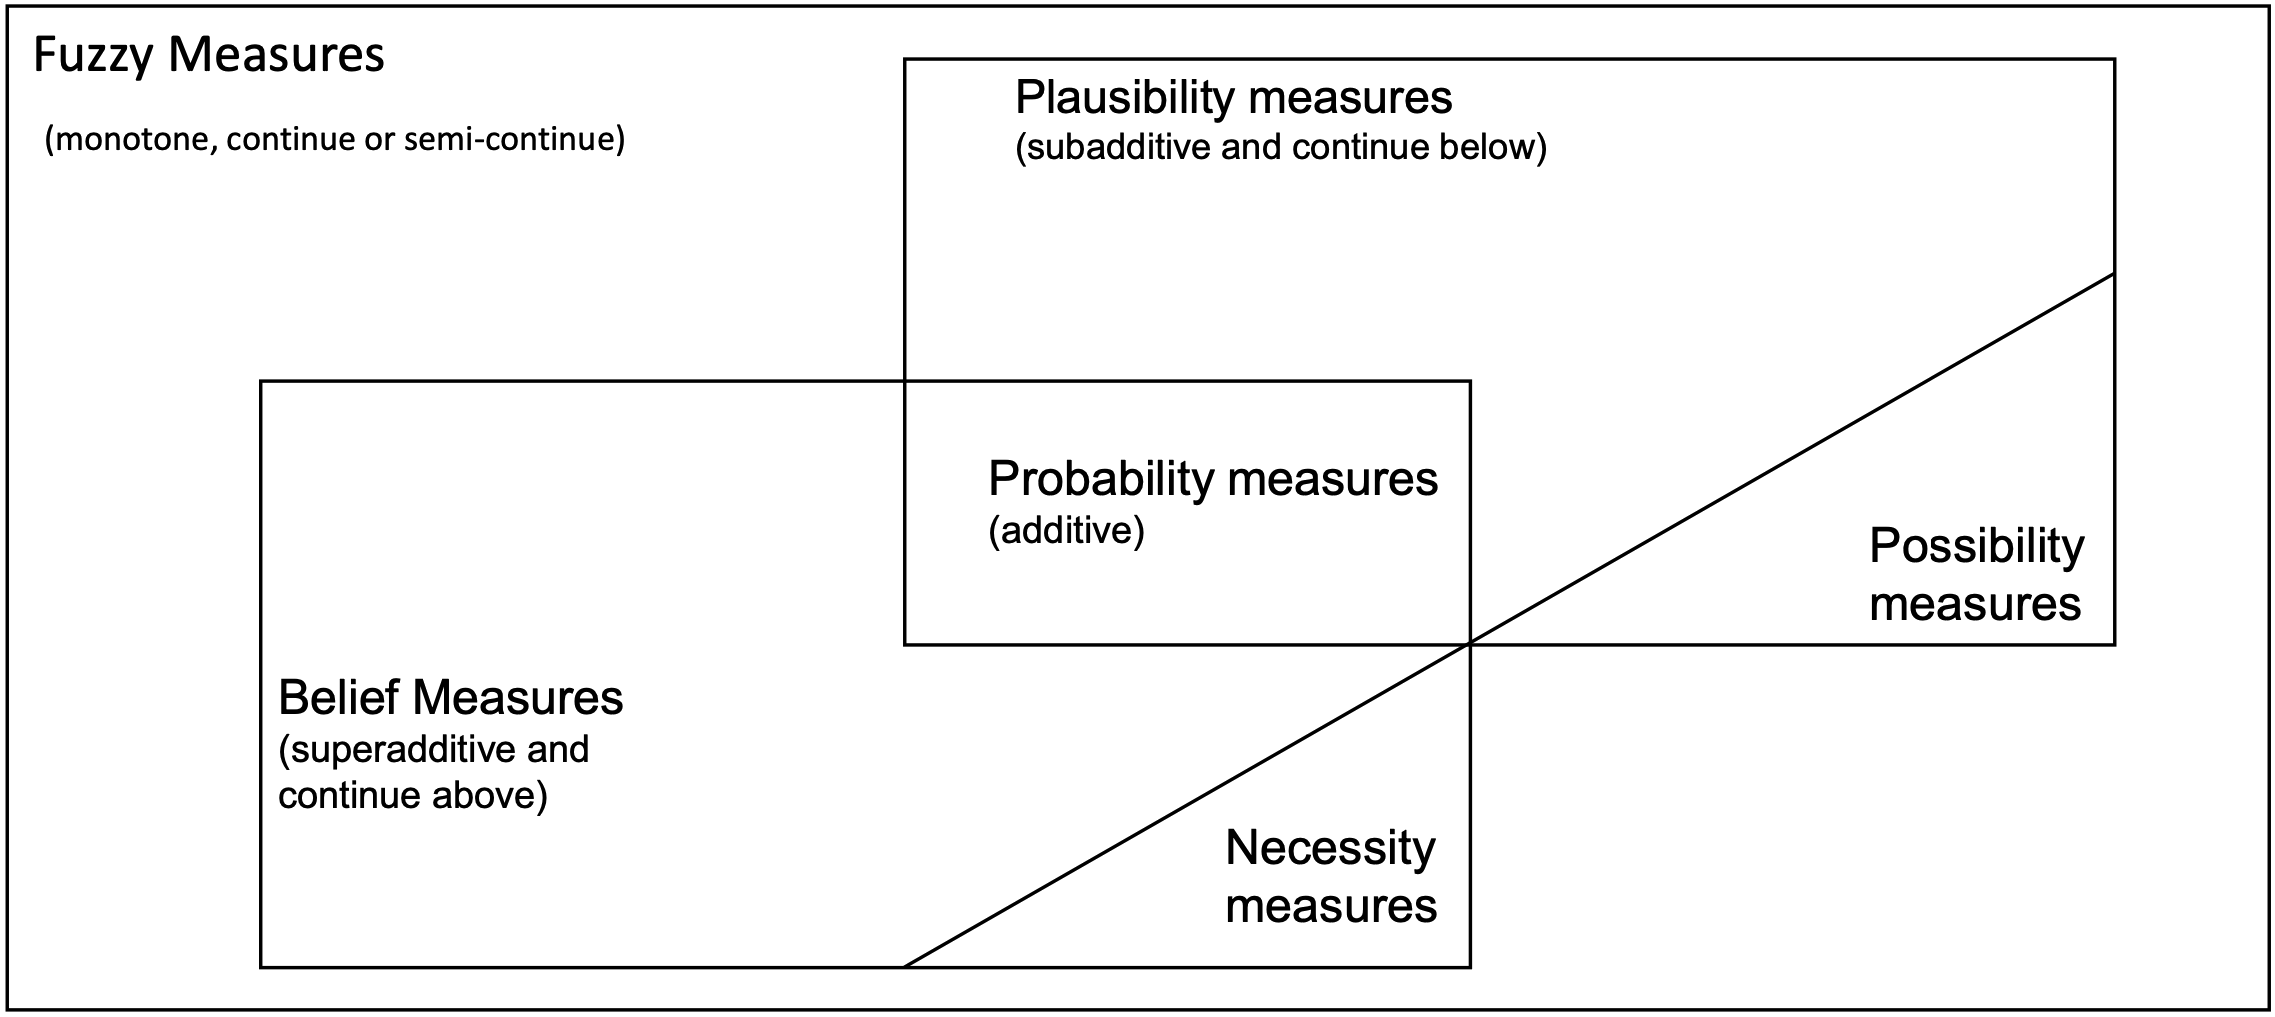
\includegraphics[width=0.75\linewidth]{images/measures.png}
        \caption{Inclusion relationships among fuzzy}
    \end{figure}

    \newpage
    \section{Fuzziness measure}
    The fuzziness measures provide the degree of fuzziness of a fuzzy set. A fuzziness measure is often quantified as the entropy of a fuzzy set.
    \begin{definition}
        Given a fuzzy set $A=\{x,\mu_A(x)\}$, the fuzziness measure (entropy) is defined as:
        \[d(A)=K \sum_{i=1}^{n}S(\mu_A(x_i))\]
        where $S(x)$ is the Shannon's function: 
        \[S(x)=-x \ln(x)-(1-x)\ln(1-x)\]
    \end{definition}
    \begin{example}
        Let's define set A as the set of integers close to ten. We have the following data:
        \begin{center}
            \begin{tabular}{|c|c|c|c|c|c|c|c|} 
            \hline
                $x$ & 7 & 8 & 9 & 10 & 11 & 12 & 13 \\ \hline
                $\mu_{\textnormal{A}(x)}$ & 0.1 & 0.5 & 0.8 & 1 & 0.8 & 0.5 & 0.1 \\ \hline
            \end{tabular}
        \end{center}
        The entropy of set A is calculated as:
        \[d(A)=0.325+0.693+0.673+0.501+0+0.501+0.693+0.325=3.711\]
        Now, let's define set B as the set of integers quite close to ten. We have the following data:
        \begin{center}
            \begin{tabular}{|c|c|c|c|c|c|c|c|c|c|} 
                \hline
                $x$         & 6     & 7     & 8     & 9     & 10    & 11    & 12    & 13    & 14 \\ \hline
                $\mu_A(x)$  & 0.1   & 0.3   & 0.4   & 0.7   & 1     & 0.8   & 0.5   & 0.3   & 0.1 \\ \hline
            \end{tabular}
        \end{center}
        The entropy of set B is calculated as:
        \[d(A)=4.35\]
        It's worth noting that set B exhibits more fuzziness compared to set A, as indicated by the fact that $d(B)>d(A)$.
    \end{example}
    
\newpage

\chapter{Probabilistic reasoning}
    \section{Basic probability}
    \begin{definition}
        A random variable, denoted as $A$, is considered a \emph{boolean-valued random variable} when it represents an event, and there exists a level of uncertainty regarding whether this event will occur.

        The concept of \emph{probability} associated with $A$ is defined as the proportion of possible outcomes or worlds in which the event represented by $A$ is true.    
    \end{definition}
    \begin{theorem}
        The fundamental axioms of probability theory are: 
        \begin{itemize}
            \item $0 \leq \textnormal{P}(A) \leq 1$. 
            \item $\textnormal{P}(A=true) = 1 \: \land \textnormal{P}(A=false) = 0\: $. 
            \item $\textnormal{P}(A \lor B)=\textnormal{P}(A)+\textnormal{P}(B)-\textnormal{P}(A \land B)$.
        \end{itemize}
    \end{theorem}
    Starting with these axioms, it becomes possible to derive various other formulas in probability theory, such as:
    \begin{enumerate}
        \item $\textnormal{P}(\overline{A})=1-\textnormal{P}(A)$.
        \item $\textnormal{P}(A)=\textnormal{P}(A \land B)+\textnormal{P}(\overline{A} \land B)$
    \end{enumerate}
    \begin{definition}
        A random variable $A$ is classified as a \emph{multivalued random variable} of arity $k$ when it can assume one of the values from the set $\{v_1, v_2, v_3, \dots, v_k\}$. 
    \end{definition}
    \begin{theorem}
        The axioms for multivalued random variable are: 
        \begin{itemize}
            \item $\textnormal{P}(A=v_i \land A=v_j) \:\:\:\:\:\: i \neq j$. 
            \item $\textnormal{P}(A=v_1 \lor A=v_2 \lor A=v_3 \lor \dots \lor A=v_k)=1$. 
        \end{itemize}
    \end{theorem}
    These new axioms enable the derivation of other valuable formulas applicable to multivalued variables:    \begin{enumerate}
        \item $\textnormal{P}(A=v_1 \lor A=v_2 \lor \dots \lor A=v_i)=\sum_{j=1}^{i}{\textnormal{P}(A=v_j)}$.
        \item $\sum_{j=1}^{k}{\textnormal{P}(A=v_j)}=1$. 
        \item $\textnormal{P}(B \land (A=v_1 \lor A=v_2 \lor \dots \lor A=v_i))=\sum_{j=1}^{i}{B \land A=v_j}$. 
        \item $\textnormal{P}(B)=\sum_{j=1}^{k}{\textnormal{P}(B \land A=v_j)}$.
    \end{enumerate}
    \begin{definition}
        The \emph{conditional probability} of event $A$ given event $B$ represents the proportion of possible scenarios where event $B$ is true, and event $A$ is true as well.
    \end{definition}
    Inference can primarily be accomplished using the following rules:
    \begin{itemize}
        \item Chain rule: $\textnormal{P}(A \land B)=\textnormal{P}(A|B)P(B)$
        \item Bayes theorem: $\textnormal{P}(A|B)=\dfrac{\textnormal{P}(B|A)\textnormal{P}(A)}{\textnormal{P}(B)}$.
        \item Sum rule (marginalization): $\textnormal{P}(A)=\sum_{b}{(A \land B=b)}$.
    \end{itemize}
    \begin{definition}
        Let's assume that $A$ and $B$ are boolean random variables. $A$ and $B$ are considered independent, denoted as $A \perp B$, if and only if:
        \[\textnormal{P}(A|B)=\textnormal{P}(A)\]

        When we have two random variables, $A$ and $B$, the joint distribution of $A$ and $B$ is represented by $\textnormal{P}(A, B)$ and encompasses the combined distribution of both variables.    
    \end{definition}
    We can represent a joint distribution of $m$ binary variables through the following steps:
    \begin{enumerate}
        \item Create a truth table listing all possible combinations of values (a total of $2^m$ entries).
        \item Calculate the probability for each combination.
        \item Verify that the sum of all probabilities equals one.
    \end{enumerate}

    \section{Probabilistic reasoning}
    Graphical models are employed to depict the factorization of joint distributions. 
    These models primarily facilitate backward reasoning, relying on Bayes' theorem. 
    When it comes to computing probabilities, graph-based algorithms play a pivotal role. 
    These algorithms operate on three main types of graphs: directed, undirected, and factor graphs.
    \begin{example}
        A perplexing murder has transpired, with two potential culprits in the spotlight: the butler and the cook. 
        The arsenal of potential murder weapons comprises a butcher's knife, a pistol, and a fireplace poker.

        Taking into account the butler's lengthy, faithful service to the family and the cook's recent hiring, along with rumors of a questionable past, we can draw the following conclusions:
        \[\textnormal{P}(\textnormal{Culprit}\rightarrow butler)=20\% \:\:\:\:\:\:\:\:\:\:\:\: \textnormal{P}(\textnormal{Culprit}\rightarrow cook)=80\%\]
        The culprit is represented as a binary random variable, with probabilities that sum to 100$\%$.

        The butler, being ex-military, maintains a firearm securely stored in a locker drawer. 
        On the other hand, the cook has easy access to a plethora of knives. 
        Additionally, it's worth noting that the butler is aging and experiencing a decline in physical strength. 
        As for the available weapons:        
        \[\textnormal{Weapon}=\{pistol,knife,poker\}\]
        Based on the provided evidence, we can assert that:
        \[\textnormal{P}(\textnormal{Weapon}|\textnormal{Culprit}\rightarrow butler)=\begin{bmatrix} 80\% & 10\% & 10\% \end{bmatrix}\]
        \[\textnormal{P}(\textnormal{Weapon}|\textnormal{Culprit}\rightarrow cook)=\begin{bmatrix} 5\% & 65\% & 30\% \end{bmatrix}\]
        
        By applying the chain rule, we can ultimately calculate the joint distribution, which is as follows:
        \begin{table}[H]
            \centering
            \begin{tabular}{c|ccc|}
            \cline{2-4}
                                                  & \textbf{pistol} & \textbf{knife} & \textbf{poker} \\ \hline
            \multicolumn{1}{|l|}{\textbf{cook}}   & $4\%$           & $52\%$         & $24\%$         \\
            \multicolumn{1}{|l|}{\textbf{butler}} & $16\%$          & $2\%$          & $2\%$          \\ \hline
            \end{tabular}
        \end{table}

        Employing the sum rule, we can determine the marginal distribution of culprits, with an 80$\%$ probability attributed to the cook and a 20$\%$ probability assigned to the butler. 
        Additionally, we can compute the marginal distribution of weapons: 20$\%$ for the pistol, 54$\%$ for the knife, and 26$\%$ for the poker.
        Should we come across the weapon at some point, we can leverage Bayes' theorem to ascertain the identity of the perpetrator.
    \end{example}

    \section{Density estimation}
    For calculating the probability of a logical expression, we can employ the following summation formula:
    \[\textnormal{P}(E)=\sum_{row \backsim E}\textnormal{P}(row)\]
    To compute inference, we can use the formula:
    \[\textnormal{P}(E_1|E_2)=\dfrac{\textnormal{P}(E_1 \land E_2)}{E_2}=\dfrac{\sum_{row \backsim E_1 \land E_2}\textnormal{P}(row)}{\sum_{row \backsim E_2}\textnormal{P}(row)}\]
    \begin{example}
        Given the following truth table: 
        \begin{table}[H]
            \centering
            \begin{tabular}{ccc|c}
            \hline
            $\boldsymbol{A}$ & $\boldsymbol{B}$ & $\boldsymbol{C}$ & $\boldsymbol{\textnormal{\textbf{P}}(A,B,C)}$ \\ \hline
            0   & 0   & 0   & 0.30       \\ 
            0   & 0   & 1   & 0.05       \\ 
            0   & 1   & 0   & 0.10       \\ 
            0   & 1   & 1   & 0.05       \\ 
            1   & 0   & 0   & 0.05       \\ 
            1   & 0   & 1   & 0.10       \\ 
            1   & 1   & 0   & 0.25       \\ 
            1   & 1   & 1   & 0.10       \\ \hline
            \end{tabular}
        \end{table}
        $\textnormal{P}(A)$ can be found by summing all the probability where $A=1$, that is: 
        \[\textnormal{P}(A) = 0.05 + 0.10 + 0.25 + 0.10 = 0.5\]
        $\textnormal{P}(A \land B)$ can be found by summing all the probability where $A=1$ and $B=1$, that is: 
        \[P(A \land B) = 0.25 + 0.10 = 0.35\]
        $\textnormal{P}(\overline{A} \lor B)$ can be found by summing all the probability where $A=0$ or $B=1$, that is: 
        \[\textnormal{P}(\overline{A} \lor B) = 0.30 + 0.05 + 0.10 + 0.05 + 0.25 + 0.10 = 0.85\]
        $P(A | B)$ can be found by dividing the probability of $A=1$ and $B=1$ by the probability where $B=1$, that is: 
        \[\textnormal{P}(A | B) = \dfrac{(0.25+0.10)}{(0.10+0.05+0.25+0.10)}=0.7\]
        $\textnormal{P}(C | A \land B)$ can be found by dividing the probability of $A=1$ and $B=1$ and $C=1$ by the probability where $A=1$ and $B=1$, that is: 
        \[\textnormal{P}(C | A \land B) = \dfrac{(0.10)}{(0.25+0.10)}=0.285\]
        $\textnormal{P}(\overline{A} | C)$ can be found by dividing the probability of $A=0$ and $C=1$ by the probability where $C=1$, that is: 
        \[\textnormal{P}(\overline{A} | C) = \dfrac{(0.05+0.05)}{(0.05+0.05+0.10+0.10)}=0.333\]
    \end{example}
    \begin{definition}
        A \emph{density estimator}  is designed to acquire knowledge in the form of a mapping from a set of attributes to a probability distribution within the attribute space, defined as:
        \[M:\{0,1\}^I \rightarrow [0,1]\]
    \end{definition}
    We can employ likelihood to assess density estimation. 
    When presented with a record $x$, a density estimator $M$ provides an estimate of how probable it is, denoted as $\widehat{\textnormal{P}}(x|M)$. 
    When dealing with a dataset containing $N$ records, a density estimator can inform us about the likelihood of the data, assuming that all records were generated independently from it:
    \[\widehat{\textnormal{P}}(\textnormal{dataset})=\widehat{\textnormal{P}}(x_1,x_2,\dots,x_N)=\prod_{n=1}^{N}\widehat{\textnormal{P}}(x|M)\]
    Due to the potential issue of likelihood values becoming extremely small, it's common practice to work with log-likelihood instead:
    \[\log{\widehat{\textnormal{P}}(\textnormal{dataset})}=\log{\prod_{n=1}^{N}{\widehat{\textnormal{P}}(x_n|M)}}=\sum_{n=1}^{N}{\log{\widehat{\textnormal{P}}(x_n|M)}}\]
    
    Density estimators offer a range of valuable capabilities, including the ability to order records by their probability, which can help identify outliers or anomalies. 
    They are also instrumental in inference tasks and can serve as a foundation for Bayes classifiers. 
    However, it's important to note that the primary challenge with joint density estimators is their susceptibility to severe overfitting.
    
    The naïve Bayes estimator model operates under the assumption that each attribute is independent of the others. 
    Using the notation where $x[i]$ represents the $i^{th}$ field of record $x$ the naïve density estimator posits that:
    \[x[i] \perp \{x[1],x[2],\dots,x[i-1],x[i],x[i+1],\dots,x[I]\}\]
    It's crucial to acknowledge that in the naïve Bayes estimator model, all attributes are treated as equally important, and the model assumes that the knowledge of one attribute conveys no information about the value of another. 
    While this final assumption is rarely accurate in real-world scenarios, it often yields effective results when applied in practice.
    \begin{example}
        In the context of the naïve Bayes estimator model, given four variables $A,B,C$, and $D$, they are all considered independent due to the model's assumptions. Consequently, this implies that:
        \[\textnormal{P}(A,\overline{B},C,\overline{D}) = \textnormal{P}(A)\textnormal{P}(\overline{B})P(C)\textnormal{P}(\overline{D})\]
    \end{example}

    In order to train a naïve Bayes estimator, we must make the assumption that $x[1],\dots,x[n]$ are independently distributed. 
    Under this hypothesis, it becomes feasible to construct any row of the resulting joint distribution as needed:
    \[\widehat{\textnormal{P}}(x[1]=u_1,x[2]=u_2,\dots,x[I]=u_I) = \prod_{k=1}^{I} \widehat{\textnormal{P}}(x[k]=u_k)\]
    \begin{table}[H]
        \centering
        \begin{tabular}{c|c|c|}
        \cline{2-3}
                                                   & \textbf{Joint estimator} & \textbf{Naïve estimator} \\ \hline
        \multicolumn{1}{|c|}{\textbf{Modelling}}   & Anything                 & Boring distributions     \\ 
        \multicolumn{1}{|c|}{\textbf{Attributes}}  & Few Boolean              & Many multivalued         \\ 
        \multicolumn{1}{|c|}{\textbf{Overfitting}} & Yes                      & Quite robust             \\ \hline
        \end{tabular}
    \end{table}
    \begin{figure}[H]
        \centering
        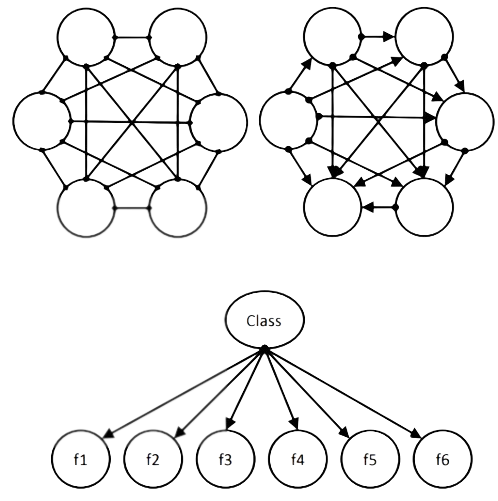
\includegraphics[width=0.35\linewidth]{images/naive-joint.png}
        \caption{Comparison between a joint and a naïve estimator}
    \end{figure}

\newpage

\chapter{Graphical models}
    \section{Introduction}
    In the real world, random variables often exhibit correlations. To address this reality, it is possible to represent a probability distribution using:
    \begin{itemize}
        \item Conditional independence assumptions that are valid for a subset of these variables.
        \item A set of conditional probabilities along with their priors.
    \end{itemize}
    Models that are constructed based on these principles are commonly referred to as graphical models.

    \section{Bayesian network}
    A Bayesian network describes the joint probability distribution of variables using a directed graph. 
    Nodes represent random variables, and edges indicate direct influence.
    \begin{example}
        In the provided Bayesian network:
        \begin{figure}[H]
            \centering
            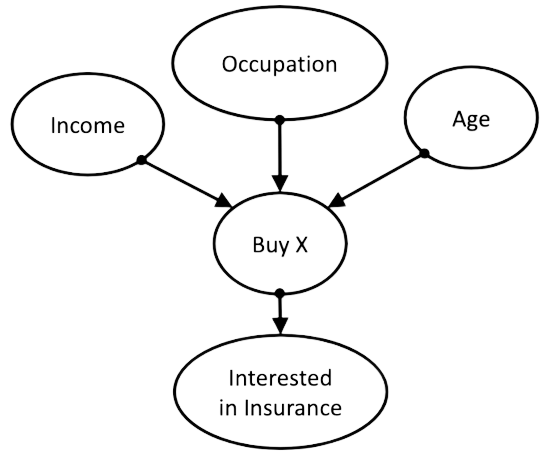
\includegraphics[width=0.25\linewidth]{images/insurance.png}
        \end{figure}
        Random variables "age," "income," and "occupation" are independent, whereas "buy X" and "Interested in insurance" are conditional probability distributions.
    \end{example}
    For a set of variables $x_1, x_2, \ldots, x_n$ we can determine any combination probability using a Bayesian network with $2^N - 1$ parameters. 
    To represent these probabilities within the network, we require only the priors and conditional parameters. 
    This is achieved by multiplying the number of nodes by $2^k$, where $k$ represents the number of incoming edges, giving us the total number of parameters needed.
    \begin{example}
        In the provided Bayesian network:
        \begin{figure}[H]
            \centering
            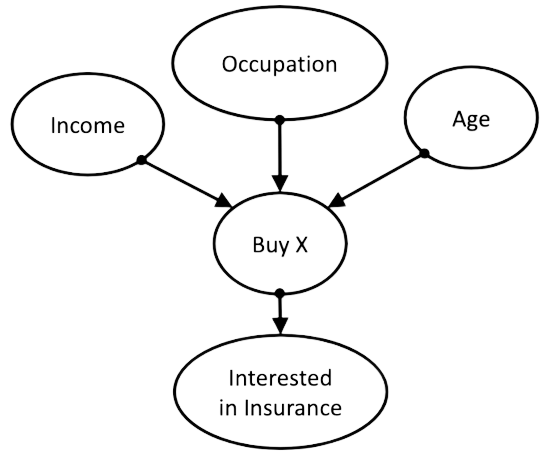
\includegraphics[width=0.25\linewidth]{images/insurance.png}
        \end{figure}
        For the full joint distribution, we require $2^N - 1$ parameters, which in this case is $2^5 - 1 = 31$ parameters.
        To represent the Bayesian network itself, we need to calculate the parameters required:
        \begin{itemize}
            \item For the "income", "occupation", and "age" nodes with no incoming edges: $3 \cdot 2^0 = 3$ parameters.
            \item For the "buy x" node with three incoming edges: $1 \cdot 2^3 = 8$ parameters.
            \item For the "Interested" node with one incoming edge: $1 \cdot 2^1 = 2$ parameters.
        \end{itemize}
        So, the total parameters needed to represent the Bayesian network is $3 + 8 + 2 = 13$ parameters.
    \end{example}
    \begin{definition}
        We define $X_1$ to be conditionally independent of $X_2$ given $X_3$ if the probability of $X_1$ is not influenced by the value of $X_2$ when we have knowledge about $X_3$.  
        This can be expressed as:
        \[\textnormal{P}(X_1|X_2,X_3)=\textnormal{P}(X_1|X_3)\]
    \end{definition}
    Likewise, for sets of variables, we can state that $X_1, X_2, X_3$ are independent of $Y_1, Y_2, Y_3$ given $Z_1,Z_2,Z_3$:
    \[\textnormal{P}(X_1,X_2,X_3|Y_1,Y_2,Y_3,Z_1,Z_2,Z_3)=\textnormal{P}(X_1,X_2,X_3|Z_1,Z_2,Z_3)\]
    \begin{example}
        Martin and Norman are tossing the same coin, and we have two variables: $A$ represents "Norman's outcome," and $B$ represents "Martin's outcome". 
        If the coin might be biased, $A$ and $B$ are not independent. 
        Observing that $B$ is heads leads us to revise our belief in $A$ being heads. 
        Therefore, we have:
        \[\textnormal{P}(A|B) \neq \textnormal{P}(A)\]
        Both variables $A$ and $B$ are dependent on another variable, $C$, representing "the coin is biased towards heads with probability $\theta$".
        Once we know the value of $C$, any evidence about $B$ cannot alter our belief about $A$.
        This can be expressed as:
        \[\textnormal{P}(A|B,C)=\textnormal{P}(A|C)\]
    \end{example}
    \begin{definition}
        A \emph{prior probability} is a probability associated with a variable that has no incoming edges in a Bayesian network. 
    \end{definition}
    It's important to note that in a Bayesian network, a node is independent of its ancestors, given its parent node.
    \begin{example}
        The event "grass is wet" ($W=true$) can be caused by two possible factors: either the "sprinkler" is on ($S=true$), or it is "raining" ($R=true$). 
        The corresponding Bayesian network is as follows.
        \begin{figure}[H]
            \centering
            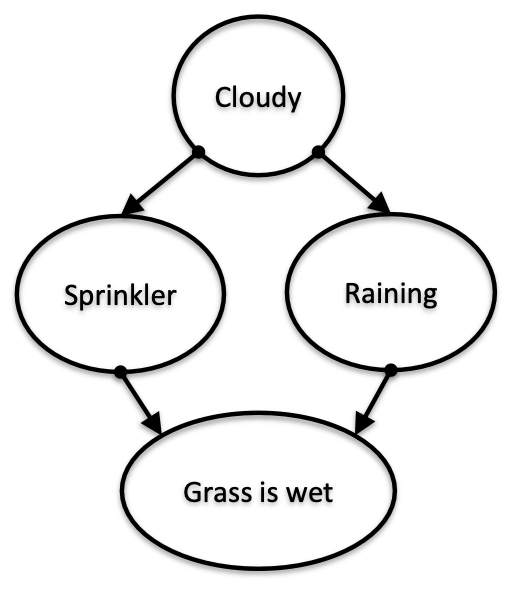
\includegraphics[width=0.25\linewidth]{images/sprinkler.png}
        \end{figure}
        Where the probabilities for cloudy are: 
        \begin{table}[H]
            \centering
            \begin{tabular}{cc}
            \hline
            \textbf{Cloudy} & \textbf{P(C)} \\ \hline
            0      & 0.5  \\
            1      & 0.5  \\ \hline
            \end{tabular}
        \end{table}
        Where the probabilities for sprinkler are: 
        \begin{table}[H]
            \centering
            \begin{tabular}{ccc}
            \hline
            \textbf{Sprinkler} & \textbf{Cloudy} & \textbf{P(S$|$C)} \\ \hline
            0         & 0      & 0.1  \\
            0         & 1      & 0.5  \\
            1         & 0      & 0.9  \\
            1         & 1      & 0.5  \\ \hline
            \end{tabular}
        \end{table}
        Where the probabilities for raining are: 
        \begin{table}[H]
            \centering
            \begin{tabular}{ccc}
            \hline
            \textbf{Raining} & \textbf{Cloudy} & \textbf{P(R$|$C)} \\ \hline
            0       & 0      & 0.8    \\
            0       & 1      & 0.5    \\
            1       & 0      & 0.2    \\
            1       & 1      & 0.5    \\ \hline
            \end{tabular}
        \end{table}
        Where the probabilities for the wet grass are: 
        \begin{table}[H]
            \centering
            \begin{tabular}{cccc}
            \hline
            \textbf{Wet} & \textbf{Sprinkler} & \textbf{Raining} & \textbf{P(W$|$S,R)} \\ \hline
            0            & 0                  & 0                & 1                   \\
            0            & 0                  & 1                & 0.1                 \\
            0            & 1                  & 0                & 0.1                 \\
            0            & 1                  & 1                & 1                   \\
            1            & 0                  & 0                & 0                   \\
            1            & 0                  & 1                & 0.9                 \\
            1            & 1                  & 0                & 0.9                 \\
            1            & 1                  & 1                & 0.99                \\ \hline
            \end{tabular}
        \end{table}
        With all these values it is possible to compute all the probabilities with the formula: 
        \[
        \begin{aligned}
            \textnormal{P}(C,S,R,W)     &= \textnormal{P}(W|S,R,C)\textnormal{P}(S,R,C)=      \\
                                        &= \textnormal{P}(W|S,R)\textnormal{P}(S,R,C)=        \\
                                        &= \textnormal{P}(W|S,R)\textnormal{P}(S|R,C)P(R,C)=  \\
                                        &= \textnormal{P}(W|S,R)\textnormal{P}(S|C)P(R,C)=    \\
                                        &= \textnormal{P}(W|S,R)\textnormal{P}(S|C)P(R|C)P(C)
        \end{aligned}
        \]
        With this formula we can compute all the joint probabilities.
        \begin{table}[H]
            \centering
            \begin{tabular}{cccc|c}
            \hline
            \textbf{C} & \textbf{S} & \textbf{W} & \textbf{R} & \textbf{P(C, S, W, R)} \\ \hline
            0          & 0          & 0          & 0          & 0.04                \\
            0          & 0          & 0          & 1          & 0                   \\
            0          & 0          & 1          & 0          & 0.001               \\
            0          & 0          & 1          & 1          & 0.009               \\
            0          & 1          & 0          & 0          & 0.036               \\
            0          & 1          & 0          & 1          & 0.324               \\
            0          & 1          & 1          & 0          & 0.0009              \\
            0          & 1          & 1          & 1          & 0.0891              \\
            1          & 0          & 0          & 0          & 0.125               \\
            1          & 0          & 0          & 1          & 0                   \\
            1          & 0          & 1          & 0          & 0.0125              \\
            1          & 0          & 1          & 1          & 0.1125              \\
            1          & 1          & 0          & 0          & 0.125               \\
            1          & 1          & 0          & 1          & 0.1125              \\
            1          & 1          & 1          & 0          & 0.00125             \\
            1          & 1          & 1          & 1          & 0.12375             \\ \hline
            \end{tabular}
        \end{table}
    \end{example}
    In statistics, the phenomenon of explaining away is often referred to as Berkson's paradox or selection bias. It pertains to situations where two variables become dependent due to the observation of a third variable. 
    In a Bayesian network, the relationships between variables can exhibit various types of dependencies and independencies: 
    \begin{itemize}
        \item $\textnormal{P}(X,Y,Z)=\textnormal{P}(X)\textnormal{P}(Y)\textnormal{P}(Z|X,Y)$ and $\textnormal{P}(X,Y|Z)=\textnormal{P}(X)\textnormal{P}(Y)$ if the nodes are connected in the following way. 
            \begin{figure}[H]
                \centering
                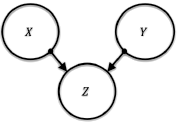
\includegraphics[width=0.2\linewidth]{images/independencies1.png}
            \end{figure}
        \item $\textnormal{P}(X,Y,Z)=\textnormal{P}(X|Z)\textnormal{P}(Y|Z)\textnormal{P}(Z)$ and $\textnormal{P}(X,Y|Z)=\textnormal{P}(X|Z)\textnormal{P}(Y|Z)$ if the nodes are connected in the following way. 
            \begin{figure}[H]
                \centering
                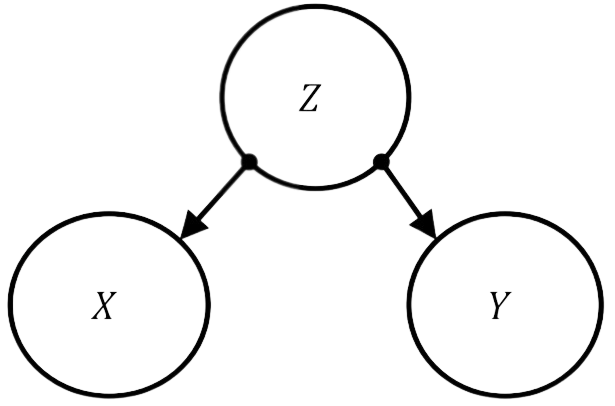
\includegraphics[width=0.2\linewidth]{images/independencies2.png}
            \end{figure}
        \item $\textnormal{P}(X,Y,Z)=\textnormal{P}(X)\textnormal{P}(Z|X)\textnormal{P}(Y|Z)$ and $\textnormal{P}(X,Y|Z)=\textnormal{P}(X|Z)\textnormal{P}(Y|Z)$ if the nodes are connected in the following way. 
            \begin{figure}[H]
                \centering
                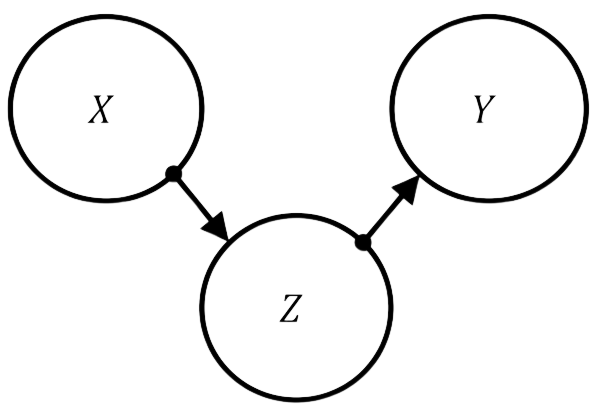
\includegraphics[width=0.2\linewidth]{images/independencies3.png}
            \end{figure}
    \end{itemize}
    \begin{definition}
        Two sets of nodes, denoted as $A$ and $B$, exhibit what is termed as \emph{conditional independence} or are often referred to as being \emph{d-separated}, given a set of nodes $C$ if and only if all paths from $A$ to $B$ are effectively blocked by the presence of $C$.
    \end{definition}
    When we classify $C$ based on its role within a Bayesian network:
    \begin{itemize}
        \item $C$ is categorized as a "root" when it remains hidden or unobserved. 
            In this scenario, the children of $C$ are dependent on each other due to the influence of a common unobserved cause. 
            However, if $C$ is observed, the children become conditionally independent, meaning that the common unobserved cause is no longer exerting an impact.
        \item $C$ is termed a "leaf" when it is hidden, and its parent nodes are marginally independent of one another. 
            Nevertheless, if $C$ (or any descendant of $C$) is observed, the parent nodes become dependent on each other, introducing conditional dependence.
        \item $C$ is described as a "bridge" when the nodes both upstream and downstream of $C$ become dependent solely when $C$ remains hidden. 
            Conditioning on $C$, by observing or introducing knowledge about it, effectively disrupts the graph's structure at that particular point, resulting in dependence between the nodes on either side of $C$.
    \end{itemize}
    These distinctions in the role of $C$ are essential in understanding how the presence or absence of observations can affect the conditional independence relationships within a Bayesian network.
    \begin{figure}[H]
        \centering
        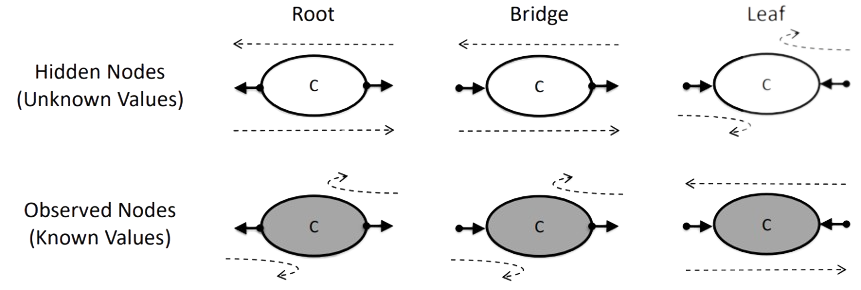
\includegraphics[width=0.75\linewidth]{images/def.png}
        \caption{Graphical representation of root, bridge, and leaf}
    \end{figure}

    Two distinct modes of reasoning are applicable when working with Bayesian networks:
    \begin{itemize}
        \item Bottom-up reasoning: this approach involves inferring the cause when provided with evidence. 
            In other words, it seeks to determine the underlying factors or causes that may have led to observed outcomes.
        \item Top-down reasoning: in this mode, we calculate the probability of one event given another event. 
            This represents a predictive utilization of Bayesian networks, as they function as "generative" models. 
            It's about estimating the likelihood of certain events based on other known events.
    \end{itemize}
    One of the most intriguing attributes of Bayesian networks is their ability to facilitate causal reasoning grounded in a robust mathematical foundation. 
    These networks allow us to explore and understand causal relationships within complex systems using a formal and structured approach.

    Moreover, Bayesian networks can encompass nodes with both continuous (real) and discrete values. 
    This versatility provides us with a diverse and powerful toolkit for constructing probabilistic models that can represent a wide range of real-world scenarios and phenomena.

    \section{Introduction}
    Inference in a Bayesian network exhibits exponential complexity, typically on the order of $O(\left\lvert X_i \right\rvert^N)$, where $\left\lvert X_i \right\rvert$ represents the cardinality of the variables involved. 
    To mitigate this computational complexity, several techniques can be applied:

    \begin{itemize}
        \item Variable elimination: this method involves systematically eliminating variables to simplify the calculation of probabilities and reduce computational complexity.
        \item Belief propagation: by passing messages between nodes in the network, this technique efficiently computes marginal probabilities and updates beliefs, helping to alleviate the computational burden.
        \item Junction trees: these data structures are used to represent Bayesian networks, and they facilitate efficient computations for probabilistic inference. 
            The process of building junction trees can significantly reduce complexity.
        \item Loopy belief propagation: in situations where the network contains loops or cycles, loopy belief propagation can be employed to approximate inferences by iteratively updating beliefs.
        \item Sampling based methods: these methods rely on random sampling to estimate probabilities and make inferences. 
            They can be effective for handling complex Bayesian networks when exact methods become impractical.
    \end{itemize}
    It's worth noting that the first three methods, namely variable elimination, belief propagation, and junction trees, are exact methods that provide precise solutions, while the last two, sampling-based methods and loopy belief propagation, are approximate techniques used when obtaining an exact solution is challenging due to computational constraints.

    \section{Variable elimination}
    The factored representation of joint probability offers an efficient approach to marginalization by consolidating summations as deeply as feasible.
    As we carry out these innermost summations, we generate fresh terms in the process.
    \begin{example}
        In the Bayesian network depicted below:
        \begin{figure}[H]
            \centering
            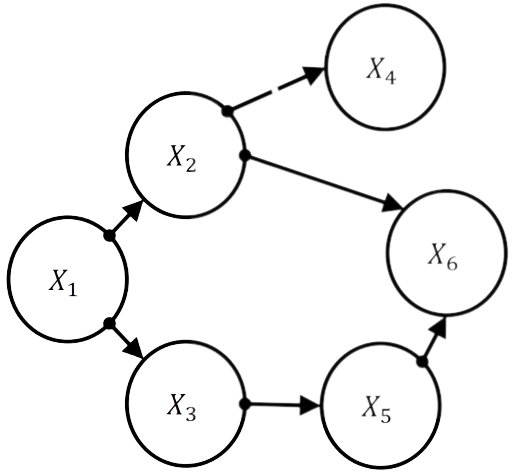
\includegraphics[width=0.25\linewidth]{images/bn.png}
        \end{figure}
        We can compute the probability distribution for $X_5$ as follows:
        \begin{align*}
            \textnormal{P}(X_5)     =& \sum_{X_1}\sum_{X_2}\sum_{X_3}\sum_{X_4}\sum_{X_6}\textnormal{P}(X_1)\textnormal{P}(X_2|X_1)\textnormal{P}(X_3|X_1)\textnormal{P}(X_4|X_2)\textnormal{P}(X_5|X_3)\textnormal{P}(X_6|X_5,X_2)          \\
                                    =& \sum_{X_1}\sum_{X_2}\sum_{X_3}\sum_{X_6}\textnormal{P}(X_1)\textnormal{P}(X_2|X_1)\textnormal{P}(X_3|X_1)\textnormal{P}(X_5|X_3)\textnormal{P}(X_6|X_5,X_2)\sum_{X_4}\textnormal{P}(X_4|X_2)          \\ 
                                    =& \sum_{X_1}\sum_{X_2}\sum_{X_3}\textnormal{P}(X_1)\textnormal{P}(X_2|X_1)\textnormal{P}(X_3|X_1)\textnormal{P}(X_5|X_3)\mu_1(X_2)\sum_{X_6}\textnormal{P}(X_6|X_5,X_2)\\
                                    =& \sum_{X_2}\sum_{X_3}\textnormal{P}(X_5|X_3)\mu_1(X_2)\mu_2(X_5,X_2)\sum_{X_1}\textnormal{P}(X_1)\textnormal{P}(X_2|X_1)\textnormal{P}(X_3|X_1)     \\
                                    =& \sum_{X_3}\textnormal{P}(X_5|X_3)\sum_{X_2}\mu_1(X_2)\mu_2(X_5,X_2)\mu_3(X_2,X_3)\\
                                    =& \sum_{X_3}\textnormal{P}(X_5|X_3)\mu_4(X_3,X_5)\\
                                    =& \mu_5(X_5)
        \end{align*}
    \end{example}
    The variable elimination procedure relies on dynamic programming. 
    To utilize this approach, we break down the main problem into multiple smaller problems by leveraging the factorization of the joint distribution. 
    This factorization not only guides us in establishing the most efficient order for variable elimination but also aids in determining the functions for the intermediate variables denoted as $\mu$.
    To automate this procedure, we employ factor graph models, a type of graphical model wherein the box notation signifies terms dependent on specific variables. 
    \begin{figure}[H]
        \centering
        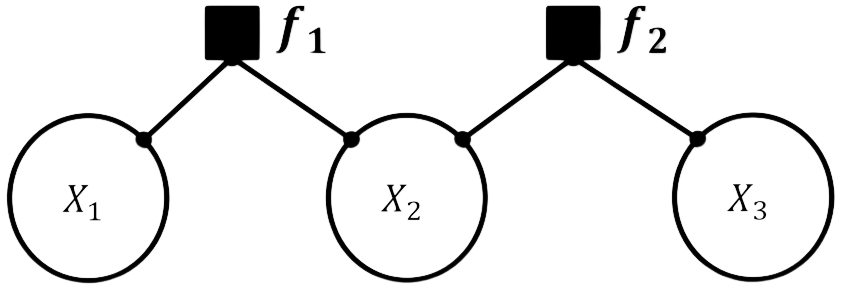
\includegraphics[width=0.25\linewidth]{images/fg.png}
        \caption{A simple example of a factor graph}
    \end{figure}
    The key characteristics of this graph include:
    \begin{itemize}
        \item It constitutes a bipartite graph.
        \item Each circular node represents a random variable, denoted as $X_i$.
        \item Each boxed node represents a factor, labeled as $f_k$, which can be expressed as a function $f_k(X_{C_k})$. 
        \item The joint probability distribution is expressed as:
            \[\textnormal{P}(X_1,X_2,\dots,X_N)=\prod_{k=1}^K{f_k(X_{C_k})}\]
    \end{itemize}
    In this representation, the factor graph serves as a powerful tool for modeling and automating probabilistic calculations, offering a clear visual depiction of variable dependencies and factor relationships.
    
    To convert a Bayesian network into a factor graph, the process involves applying a step called moralization. 
    In the typical scenario, this operation entails establishing links between the parents of nodes while preserving as many independence properties as possible.
    \begin{figure}[H]
        \centering
        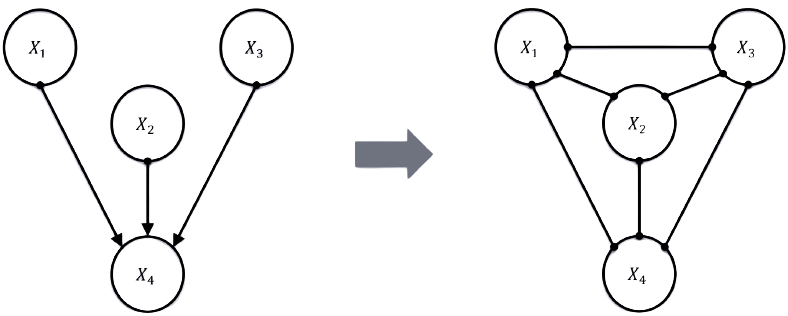
\includegraphics[width=0.5\linewidth]{images/mor.png}
        \caption{An example of moralization}
    \end{figure}
    To convert the Bayesian network into a factor graph, it's necessary to combine unconnected parents into a single factor.
    \begin{example}
        In the provided Bayesian network:
        \begin{figure}[H]
            \centering
            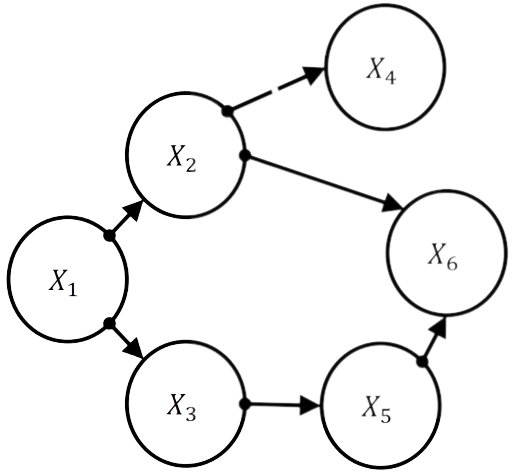
\includegraphics[width=0.25\linewidth]{images/bn.png}
        \end{figure}
        The corresponding factor graph is represented as follows:
        \begin{figure}[H]
            \centering
            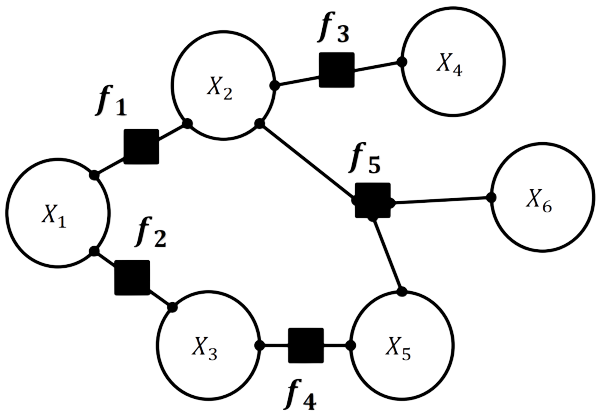
\includegraphics[width=0.25\linewidth]{images/bnf.png}
        \end{figure}
    \end{example}
    \begin{definition}
        A graph is a \emph{perfect map} if and only if every independence property of a distribution is reflected in the graph and vice versa. 
    \end{definition}
    Please be aware of the following:
    \begin{itemize}
        \item Not all probability distributions can be faithfully depicted using directed or undirected graphs.
        \item Not all directed graphs can be transformed into undirected graphs while maintaining their original properties.
        \item Not all undirected graphs can be converted into directed graphs while preserving their original characteristics.
    \end{itemize}
    \begin{example}
        The chain can be portrayed as a factor graph in the following manner:
        \begin{figure}[H]
            \centering
            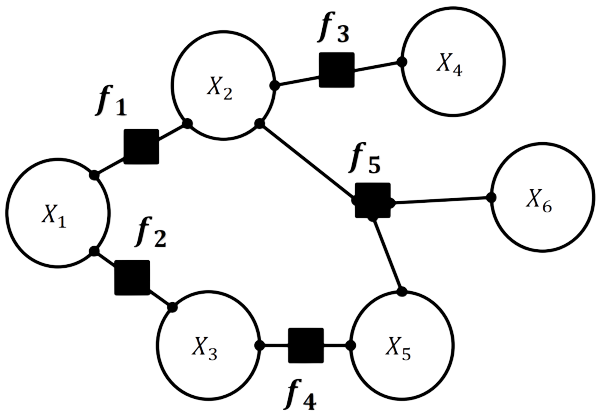
\includegraphics[width=0.3\linewidth]{images/bnf.png}
        \end{figure}
        \begin{itemize}
            \item $f_1(X_1)=P(X_1)$
            \item $f_2(X_1,X_2)=\textnormal{P}(X_1|X_2)$
            \item $f_3(X_2,X_3)=\textnormal{P}(X_3|X_2)$
            \item $f_4(X_3,X_4)=\textnormal{P}(X_4|X_3)$
            \item $f_5(X_4,X_5)=\textnormal{P}(X_5|X_4)$
            \item $f_5(X_5,X_6)=\textnormal{P}(X_6|X_5)$
        \end{itemize}
    \end{example}
    It's important to note that factor graphs are not unique; there are various ways to represent any given Bayesian network.

    The variable elimination algorithm takes two inputs: a list denoted as $F$ containing factors and a tuple labeled as $C_0$ representing the output variables to retain. 
    The result of the algorithm is a single factor $m$ that encompasses the variables in $X_{C_0}$.
    \begin{algorithm}[H]
        \caption{Variable elimination algorithm}
            \begin{algorithmic}[1]
                \State define all variables present in $F$ as $V\leftarrow\textnormal{vars}(F)$
                \State define all variables to be eliminated as $E\leftarrow V-C_0$
                \For {all $i \in E$}
                    \State call eliminate$\_$single$\_$variable$(F,i)$
                \EndFor
                \For {all remaining factors}
                    \State $m \leftarrow \prod_{f \in F}f$
                \EndFor
            \end{algorithmic}
    \end{algorithm}
    The function eliminate$\_$single$\_$variable$(F,i)$ in the prior algorithm accepts as inputs the list of factors denoted as $F$ and the variable identified by $i$. 
    It returns the updated list of factors, which remains labeled as $F$.
    \begin{algorithm}[H]
        \caption{eliminate$\_$single$\_$variable$(F,i)$}
            \begin{algorithmic}[1]
                \State find relevant subset $f \subset F$ of factors over $i$ as $f \leftarrow\{C|i\in C\}$
                \State define the remaining clique as $C_t \leftarrow \textnormal{vars}(f)-\{i\}$
                \State compute the temporary factor as $\mu(X_{C_t})=\sum_{X_i}\prod_{f \in F}f$
                \State remove old factors $f$ and append new temporary factor $t$ to $F$
                \State \Return $F$
            \end{algorithmic}
    \end{algorithm}
    \begin{example}
        Consider the Bayesian network illustrated below:
        \begin{figure}[H]
            \centering
            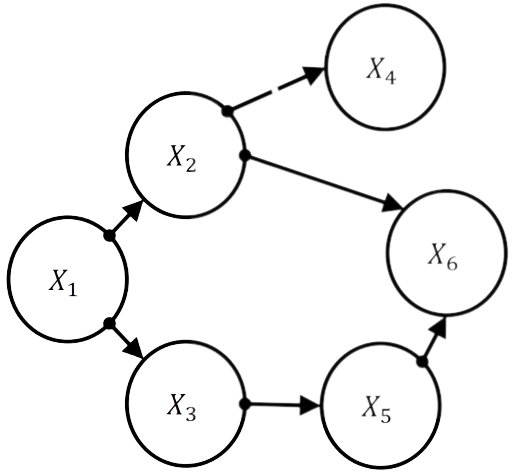
\includegraphics[width=0.25\linewidth]{images/bn.png}
        \end{figure}
        We can compute the factor graph with moralization, resulting in the following factor graph:
        \begin{figure}[H]
            \centering
            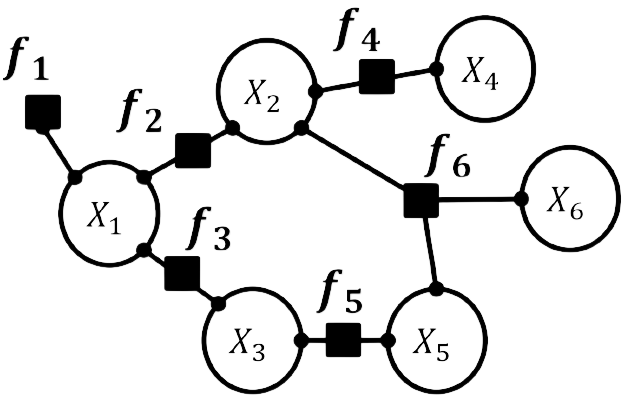
\includegraphics[width=0.25\linewidth]{images/bnf1.png}
        \end{figure}
        Now, let's compute the marginal probability $\textnormal{P}(X_1,X_6)=\mu(X_1,X_6)$. To do this, we'll utilize the variable elimination algorithm with the following inputs:
        \begin{itemize}
            \item $F=\{f_1,f_2,f_3,f_4,f_5,f_6\}$
            \item $C_0=\{X_1,X_6\}$
        \end{itemize}
        The algorithm progresses as follows:
        \begin{enumerate}
            \item Define all the variables present in $F$: 
                \[V=\{X_1,X_2,X_3,X_4,X_5,X_6\}\]
            \item Calculate the set of variables to be eliminated:
                \[E=V-C_0=\{X_1,X_2,X_3,X_4,X_5,X_6\}-\{X_1,X_6\}=\{X_2,X_3,X_4,X_5\}\]
        \end{enumerate}
        Now, we need to eliminate the single variables contained in set $E$ using the  eliminate$\_$single$\_$variable function. Here's the step-by-step process for each variable:
        \begin{itemize}
            \item Eliminate $X_4$: 
                \begin{itemize}
                    \item Check the connected functions: $f=\{f_4\}$. 
                    \item The clique containing $X_4$ (excluding itself) is: $C_t=\{X_2\}$. 
                    \item Calculate the temporary factor: $\mu_1(X_2)=\sum_{X_4}P(X_4|X_2)$. 
                    \item Update $F$ to: $F=\{f_1,f_2,f_3,f_5,f_6,\mu_1\}$. 
                    \item Remove $f$ from $E$, resulting in $E=\{X_2,X_3,X_5\}$
                \end{itemize}
            \item Eliminate $X_3$: 
                \begin{itemize}
                    \item Check the connected functions: $f=\{f_3,f_5\}$. 
                    \item The clique containing $X_3$ (excluding itself) is: $C_t=\{X_1,X_5\}$. 
                    \item Calculate the temporary factor: $\mu_2(X_1,X_5)=\sum_{X_3}P(X_3|X_1)P(X_5|X_3)$. 
                    \item Update $F$ to: $F=\{f_1,f_2,f_6,\mu_1,\mu_2\}$. 
                    \item Remove $f$ from $E$, resulting in $E=\{X_2,X_5\}$
                \end{itemize}
            \item Eliminate $X_5$: 
                \begin{itemize}
                    \item Check the connected functions: $f=\{f_6,\mu_2\}$. 
                    \item The clique containing $X_5$ (excluding itself) is: $C_t=\{X_1,X_2,X_6\}$. 
                    \item Calculate the temporary factor: $\mu_3(X_1,X_2,X_6)=\sum_{X_5}\mu_2(X_1,X_5)P(X_6|X_2,X_5)$. 
                    \item Update $F$ to: $F=\{f_1,f_2,\mu_1,\mu_3\}$. 
                    \item Remove $f$ from $E$, resulting in $E=\{X_2\}$
                \end{itemize}
            \item Eliminate $X_2$: 
                \begin{itemize}
                    \item Check the connected functions: $f=\{f_2,\mu_1,\mu_3\}$. 
                    \item The clique containing $X_2$ (excluding itself) is: $C_t=\{X_1,X_6\}$. 
                    \item Calculate the temporary factor: $\mu_4(X_1,X_6)=\sum_{X_2}\mu_1(X_2)P(X_2|X_1)\mu_3(X_1,X_2,X_6)$. 
                    \item Update $F$ to: $F=\{f_1,\mu_4\}$. 
                    \item Remove $f$ from $E$, resulting in $E=\varnothing$
                \end{itemize}
        \end{itemize}
        After these iterations, we have the following results:
        \begin{itemize}
            \item $F=\{f_1,\mu_4\}$
            \item $C_0=\{X_1,X_6\}$
        \end{itemize}
        The final steps involve multiplying all the elements in $f$: 
        \[\textnormal{P}(X_1,X_6)=\mu_4 \cdot f_1=P(X_1)\mu_4(X_1,X_6)\]
        This yields the marginal probability $\textnormal{P}(X_1,X_6)$ using the variable elimination algorithm.
    \end{example}
    It's worth mentioning that the order in which variables are selected as input for the function can be determined using a heuristic function. 
    One common approach is to order the nodes based on the ascending number of connections they have in the factor graph.
    \begin{example}
        Given the Bayesian network and the associated truth tables:
        \begin{figure}[H]
            \centering
            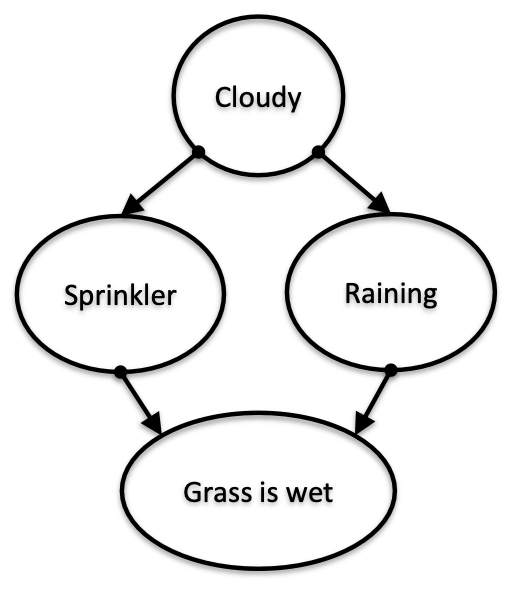
\includegraphics[width=0.3\linewidth]{images/sprinkler.png}
        \end{figure}
        \begin{table}[H]
            \centering
            \begin{tabular}{cc}
            \hline
            \textbf{Cloudy} & \textbf{P(C)} \\ \hline
            0      & 0.5  \\
            1      & 0.5  \\ \hline
            \end{tabular}
        \end{table}
        \begin{table}[H]
            \centering
            \begin{tabular}{ccc}
            \hline
            \textbf{Sprinkler} & \textbf{Cloudy} & \textbf{P(S$|$C)} \\ \hline
            0         & 0      & 0.1  \\
            0         & 1      & 0.5  \\
            1         & 0      & 0.9  \\
            1         & 1      & 0.5  \\ \hline
            \end{tabular}
        \end{table}
        \begin{table}[H]
            \centering
            \begin{tabular}{ccc}
            \hline
            \textbf{Raining} & \textbf{Cloudy} & \textbf{P(R$|$C)} \\ \hline
            0       & 0      & 0.8    \\
            0       & 1      & 0.5    \\
            1       & 0      & 0.2    \\
            1       & 1      & 0.5    \\ \hline
            \end{tabular}
        \end{table}
        \begin{table}[H]
            \centering
            \begin{tabular}{cccc}
            \hline
            \textbf{Wet} & \textbf{Sprinkler} & \textbf{Raining} & \textbf{P(W$|$S,R)} \\ \hline
            0            & 0                  & 0                & 1                   \\
            0            & 0                  & 1                & 0.1                 \\
            0            & 1                  & 0                & 0.1                 \\
            0            & 1                  & 1                & 1                   \\
            1            & 0                  & 0                & 0                   \\
            1            & 0                  & 1                & 0.9                 \\
            1            & 1                  & 0                & 0.9                 \\
            1            & 1                  & 1                & 0.99                \\ \hline
            \end{tabular}
        \end{table}
        We want to compute $\textnormal{P}(W)$. To do this, we start by transforming the Bayesian network into a factor graph, where we define the factors as follows:
        \begin{itemize}
            \item $f_1(C)=\textnormal{P}(C)$.
            \item $f_2(S,C)=\textnormal{P}(S|C)$.
            \item $f_3(R,C)=\textnormal{P}(R|C)$.
            \item $f_4(W,S,R)=\textnormal{P}(W|S,R)$.
        \end{itemize}
        The resulting factor graph looks like this:
        \begin{figure}[H]
            \centering
            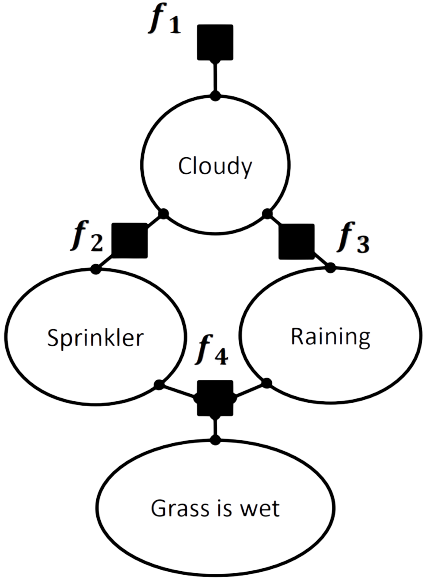
\includegraphics[width=0.25\linewidth]{images/sprinklerfg.png}
        \end{figure} 
        After applying the variable elimination algorithm, we obtain the following graph:
        \begin{figure}[H]
            \centering
            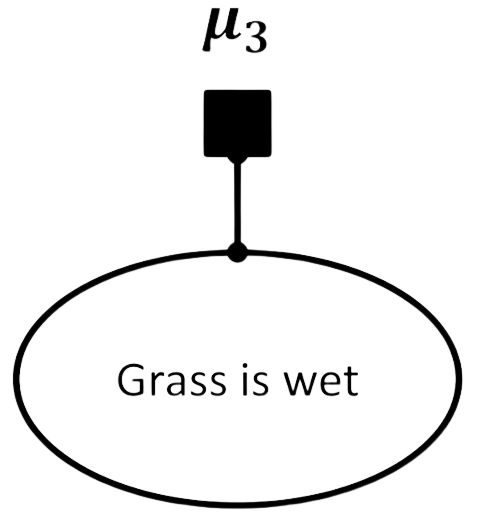
\includegraphics[width=0.15\linewidth]{images/fg1.png}
        \end{figure} 
        The corresponding truth table for the variable $\mu_3(W)$ is as follows:
        \begin{table}[H]
            \centering
            \begin{tabular}{cc}
            \hline
            \textbf{Wet} & \textbf{$\boldsymbol{\mu_3}$(W)} \\ \hline
            0      & 0.22915  \\
            1      & 0.77085  \\ \hline
            \end{tabular}
        \end{table}
    \end{example}
    Variable elimination possesses several advantages, including its simplicity of implementation and the faithful representation of manual calculations. 
    With an optimal ordering, its complexity is $O(N2^K)$.
    However, it does have its drawbacks. 
    Finding the optimal ordering is an $\mathcal{NP}$-hard problem, it can compute only one marginal at a time, and computing all marginals necessitates $N$ executions, which can be inefficient for more extensive networks.

    \section{Belief propagation}
    Belief propagation, also called message passing, is similar to variable elimination. 
    This algorithm can be run in parallel at each node, where it computes the message set to the variable from the factor and from the variable to the factor. 
    It is based on two steps: compute messages and then compute probabilities from the obtained messages. 
    Circular dependencies can be solved if the graph is a tree or polytree (tree with no root). 

    Note that messages correspond to $\mu$ factors in the variable elimination algorithm. 
    Leaves $\mu$ factors are always 1.
    Since to start the algorithm we need the values of messages from a previous state, we can start from the leaves. 

    As we said, belief propagation can be written as a parallel procedure that follows these steps: 
    \begin{enumerate}
        \item Initialize all messages as one $\mu_{f_s\rightarrow X_i}= 1$ and $\mu_{X_i \rightarrow f_s}= 1$. 
        \item Update all messages: 
            \[\mu_{f_s\rightarrow X_i}^{new}(X_i)=\sum_{X_s \backslash X_i}f_s(X_i,X_s)\prod_{X_j \in new(X_i), j \neq i}\mu_{X_i \rightarrow f_s}^{old}(X_j)\]
            \[\mu_{X_i \rightarrow f_s}^{new}(X_i)=\prod_{f_l \in new(X_i),f_l \neq f_s}\mu_{f_l \rightarrow X_i}^{old}(X_i)\]
        \item Update believes: 
            \[b_{f_s}(X_s)=f_s(X_s) \prod_{j \in f_s}\mu_{X_j \rightarrow f_s}(X_j)\]
            \[b_{X_i}(X_i)=\prod_{f_s \in new(i)}\mu_{f_s \rightarrow X_i}(X_i)\]
    \end{enumerate}
    We iterate this procedure until convergence. 
    \begin{example}
        SLIDE 61 in poi
    \end{example}







\end{document}